\chapter{Reticulados}
\label{cap:reticulados}
%https://repositorio.unifesp.br/bitstream/handle/11600/60730/Lucas_Eduardo_Trabalho_de_Graduacao_Final.pdf?sequence=7&isAllowed=y

    Reticulados são objetos geométricos que podem ser descritos como pontos de uma grade regular n-dimensional \cite{daniele-lattices}. Esta estrutura tem sido alvo de pesquisadores da área da criptografia devido a problemas computacionais de difícil resolução tanto para computadores convencionais quanto para computadores quânticos. Tais problemas computacionais foram utilizados na construção de sistemas criptográficos como \ac{ML-KEM} \cite{kyber}, Dilithium \cite{dilithium}, NTRU \cite{ntru} e FALCON \cite{falcon}. Este capítulo é dedicado ao estudo e aplicabilidades dos reticulados na área da criptografia.

\begin{definition}[reticulado]
    Um reticulado $\mathcal{L}$ é um subgrupo aditivo discreto de $\mathbb{R}^{n}$, ou seja, satisfaz as seguintes propriedades:

    \begin{itemize}
        \item[(i)] fechado para adição: $\forall x,y \in \mathcal{L},\ x+y \in \mathcal{L}$;
        \item[(ii)] discreto: $\forall x,y \in \mathcal{L}$, em que $x \neq y$, existe um valor $\epsilon > 0$ tal que a distância entre eles é $\lVert x-y \rVert \ge \epsilon$.
    \end{itemize}
\end{definition}

    As Figuras \ref{fig:lattice-2d} e \ref{fig:lattice-3d} ilustram um exemplo de um reticulado de duas dimensões e três dimensões respectivamente.
    
    \begin{figure}[htb!]
        \begin{minipage}[c]{0.5\linewidth}
            \centering
            \caption{Reticulado de duas dimensões.}
            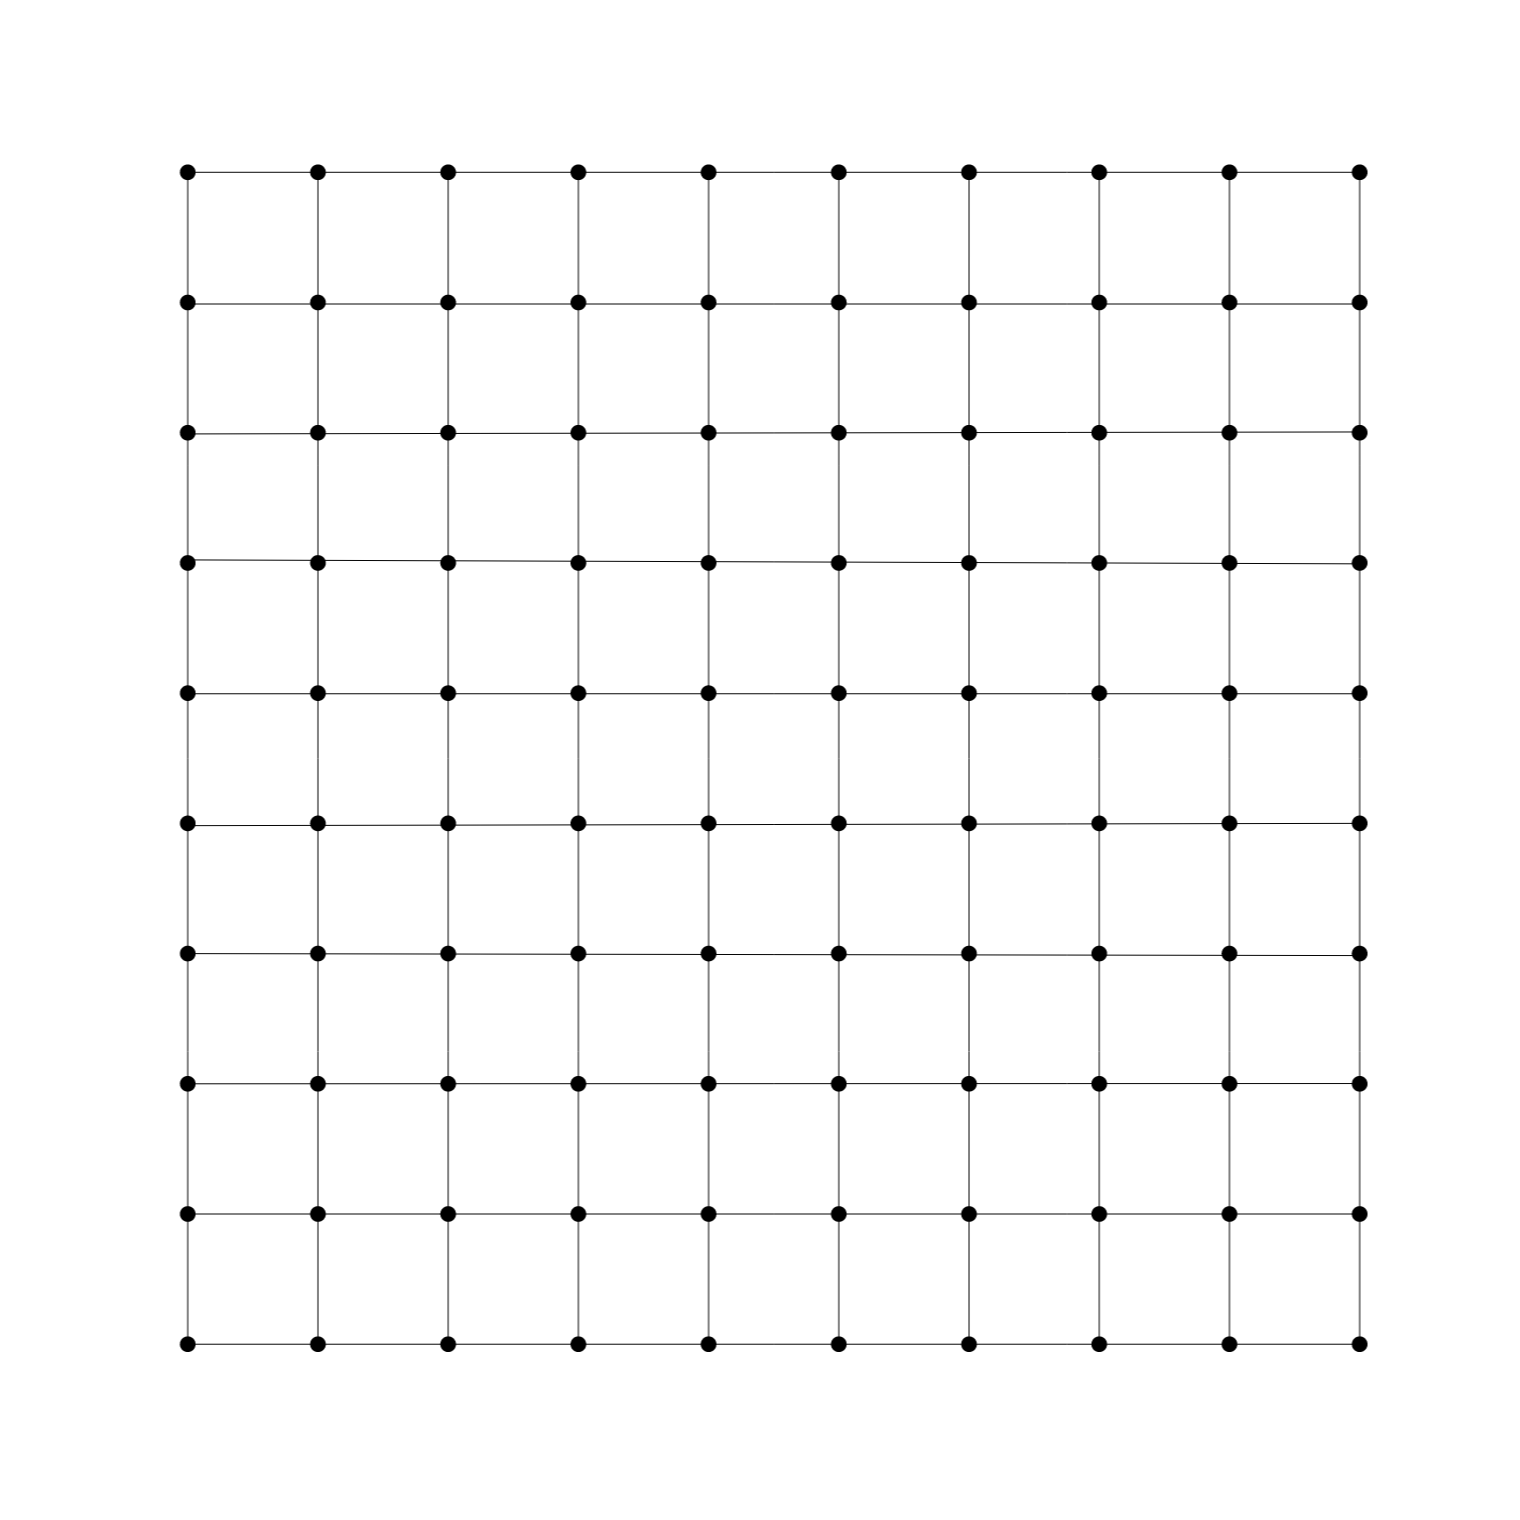
\includegraphics[width=0.75\textwidth]{Figuras/lattice-2d.png}\\
            \footnotesize{Fonte: O autor.}
            \label{fig:lattice-2d}
        \end{minipage}\hfill
        \begin{minipage}[c]{0.5\linewidth}
            \centering
            \caption{Reticulado de três dimensões.}
            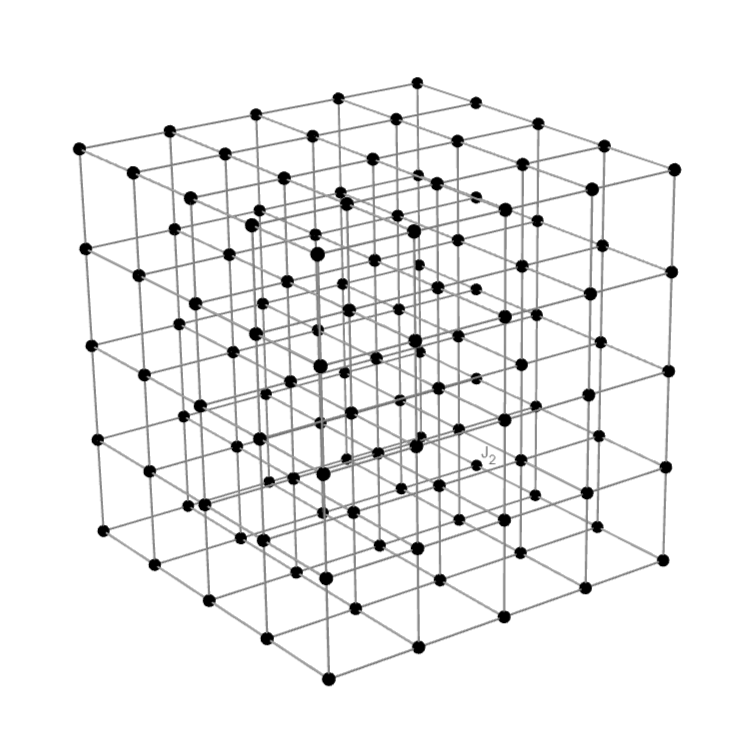
\includegraphics[width=0.75\textwidth]{Figuras/lattice-3d.png}\\
            \footnotesize{Fonte: O autor.}
            \label{fig:lattice-3d}
        \end{minipage}
    \end{figure}


\section{Base de um reticulado}
    %estou usando d para quantidade de vetores e para quantidade de componentes
    Assim como os espaços vetoriais podem ser representados/gerados por uma combinação linear entre vetores linearmente independentes, os reticulados também, com exceção que os coeficientes da combinação linear devem pertencer ao conjunto $\mathbb{Z}$, o que faz com que esta estrutura seja regular \cite{daniele-lattices}. A definição de um reticulado $\mathcal{L(\beta)}$, gerado por uma base $\beta = \{b_0, b_1, ... , b_{n-1}\} \subset \mathbb{R}^{n}$, é expressa por: 
    
    $$\mathcal{L(\beta)} = \Biggl\{\sum_{i=0}^{n-1} m_i b_i\ |\ m_i\in\mathbb{Z},\ b_i \in \beta \Biggl\},$$

    Um elemento de um reticulado, por sua definição, é representado por um vetor ou ponto. Entretanto, devido aos isomorfismos aditivos $\sigma_1$ e $\sigma_2$, é possível representar os elementos de um reticulado na forma polinomial ou matricial respectivamente. A representação de um elemento na forma polinomial possui mais utilidade em alguns problemas específicos envolvendo reticulados como \ac{RLWE} e \ac{MLWE}.
    
    $\begin{array}{rl}
        \sigma_1 &:P[x] \to \mathbb{Z}^n\\
               &:a_0 + a_1 x + a_2 x^2 + ... + a_{n-1} x^{n-1} \to (a_0, a_1, a_2, ... , a_{n-1})
    \end{array}$\\\\

    $\begin{array}{rl}
        \sigma_1^{-1} &:\mathbb{Z}^n \to P[x]\\
               &:(a_0, a_1, a_2, ... , a_{n-1}) \to a_0 + a_1 x + a_2 x^2 + ... + a_{n-1} x^{n-1}
    \end{array}$\\\\

    Através do isomorfismo $\sigma_1$ é possível transformar um polinômio na forma $a_0 + a_1 x + a_2 x^2 + ... + a_{n-1} x^{n-1}$ em um ponto ou vetor na forma $(a_0, a_1, a_2, ... , a_{n-1})$. O inverso desse isomorfismo, representado por $\sigma_1^{-1}$, realiza o mapeamento inverso, transformando um ponto em um polinômio. Por outro lado, a representação de um elemento de um reticulado na forma matricial facilita a visualização na realização dos cálculos dos principais problemas computacionais sobre esta estrutura.
    
    $\begin{array}{rl}
            \sigma_2 &:M_n \to \mathbb{Z}^n\\
                   &:[a_0\ a_1\ a_2\ ...\ a_{n-1}] \to (a_0, a_1, a_2, ... , a_{n-1})
    \end{array}$\\\\

    $\begin{array}{rl}
            \sigma_2^{-1} &:\mathbb{Z}^n \to M_n\\
                   &:(a_0, a_1, a_2, ... , a_{n-1}) \to [a_0\ a_1\ a_2\ ...\ a_{n-1}]
    \end{array}$\\\\

    O isomorfismo aditivo $\sigma_2$ e sua inversa $\sigma_2^{-1}$, por sua vez, transformam uma matriz linha ou coluna em um elemento de $\mathbb{Z}^n$ e vice-versa. Estes isomorfismos aditivos significam que um elemento de um reticulado representado por um ponto, vetor, matriz ou polinômio, possui o mesmo comportamento com relação à operação de adição.

    Uma base $\beta = \{b_0, b_1, ... b_{n-1}\} \subset \mathbb{R}^{n}$ de um reticulado também pode ser representada na forma matricial devido ao isomorfismo $\sigma_2$, na qual as componentes dos vetores da base formam as colunas da matriz geradora do reticulado. Seja $\textbf{B} = [b_0\ b_1\ ...\ b_{n-1}] \in \mathbb{R}^{d \times n}$ a base do reticulado $\mathcal{L}$ na forma matricial, $\mathcal{L}(\textbf{B})$ pode ser representada por:

    $$\mathcal{L}(\textbf{B}) = \{\textbf{B}x\ |\ x \in \mathbb{Z}^n\},$$

    \noindent
    em que $\textbf{B}x$ é uma multiplicação matricial usual, $d$ representa o número de componentes dos vetores de $\textbf{B}$ e $n$ representa a dimensão do reticulado $\mathcal{L}(\textbf{B})$. Quando o número de componentes dos vetores da base de um reticulado coincide com seu grau, ou seja, a base do reticulado na forma matricial possui posto completo\footnote{Em outras palavras: tem-se uma matriz quadrada.}, o reticulado é dito completo.

    Ambas as formas de representação de um reticulado são equivalentes, isso pode ser verificado derivando a notação por combinação linear a partir da notação matricial:

    \begin{center}
        $\begin{bmatrix}
                b_{0 0} & b_{0 1} & . & . & . & b_{0 (n-1)}\\
                b_{1 0} & b_{1 1} & . & . & . & b_{1 (n-1)}\\
                b_{2 0} & b_{2 1} & . & . & . & b_{2 (n-1)}\\
                .      & .      & . &   &   & .     \\
                .      & .      &   & . &   & .     \\
                .      & .      &   &   & . & .     \\
                b_{(d-1) 0} & b_{(d-1) 1} &   &   &   & b_{(d-1) (n-1)}
            \end{bmatrix}$
        %
        $\begin{bmatrix}
            x_0\\
            x_1\\
            x_2\\
            .  \\
            .  \\
            .  \\
            x_{n-1}
        \end{bmatrix}$
        %
        $\Leftrightarrow$\\
    \end{center}

    \begin{center}
        $x_0\begin{bmatrix} b_{00} \\ b_{01} \\ b_{02} \\ . \\ . \\ . \\ b_{0 (d-1)} \end{bmatrix}$ + 
        $x_1\begin{bmatrix} b_{10} \\ b_{11} \\ b_{12} \\ . \\ . \\ . \\ b_{1 (d-1)} \end{bmatrix}$ +
        $x_2\begin{bmatrix} b_{20} \\ b_{21} \\ b_{22} \\ . \\ . \\ . \\ b_{2 (d-1)} \end{bmatrix}$ + ... +
        $x_{n-1}\begin{bmatrix} b_{(n-1) 0} \\ b_{(n-1) 1} \\ b_{(n-1) 2} \\ . \\ . \\ . \\ b_{(n-1) (d-1)} \end{bmatrix}$
        %
        $\Leftrightarrow$\\
    \end{center}

    \begin{center}
        $x_0 \vec{b_0} + x_1 \vec{b_1} + x_2 \vec{b_2} + ... + x_{n-1} \vec{b_{n-1}}$
    \end{center}

    Existem alguns tipos de reticulados que devem ser mencionados para melhor compreensão dos conceitos utilizados posteriormente neste trabalho.

    \begin{definition}[reticulado inteiro]
        Um reticulado $\mathcal{L}(\textbf{B})$ é dito inteiro se os coeficientes dos vetores da base $\textbf{B}$ forem inteiros, ou seja, $\mathcal{L}(\textbf{B}) = \{\textbf{B}x\ |\ \textbf{B} \in \mathbb{Z}^{d \times n},\ x \in \mathbb{Z}^n\}$.
    \end{definition}

    %https://simons.berkeley.edu/sites/default/files/docs/14953/intro.pdf
    \begin{definition}[reticulado dual]
        A dual de um reticulado $\mathcal{L}$, denotado por $\mathcal{L}^{*}$, é o conjunto de todos os vetores $\vec{x} \in span(\mathcal{L})$ tal que $\langle \vec{x},\vec{y} \rangle \in \mathbb{Z}$, para todo $\vec{y} \in \mathcal{L}$.
    \end{definition}

    \begin{definition}[reticulado ideal]
    \label{ideal_lattice}
        Seja um anel $A$ e um isomorfismo aditivo $\sigma$ que mapeia $A$ para $\sigma (A) \subset \mathbb{R}^n$. Um reticulado ideal é um $\sigma(I)$ para um ideal $I \subseteq A$ \cite{ring_lwe}.
    \end{definition}

    Segundo a Definição \ref{ideal_lattice}, um reticulado ideal é obtido aplicando um isomorfismo aditivo que mapeia um ideal para um subconjunto de $\mathbb{R}^n$. A estrutura $\mathbb{Z}{[}x{]}/ \langle x^n + 1 \rangle$, na qual é abordada na Seção \ref{cap:lattice_problems} e pode ser consultada no Apêndice \ref{ap:conceitos_matematicos}, representa a um reticulado ideal, visto que existe um isomorfismo aditivo que mapeia um polinômio pertencente ao ideal $\langle x^n + 1 \rangle$ para um subconjunto de $\mathbb{R}^n$, neste caso $\mathbb{Z}^n$.

    \begin{definition}[reticulado modular]
    \label{modular_lattice}
        Seja um anel $A$ e um isomorfismo aditivo $\sigma$ que mapeia $A$ para $\sigma (A) \subset \mathbb{R}^n$. Um reticulado modular é definido por uma função que mapeia um conjunto $\{ \sigma(A)_1,\sigma(A)_2,...,\sigma(A)_d \}$ para $\mathbb{R}^{nd}$ \cite{module-lwe}. 
    \end{definition}

    Um reticulado modular é um subconjunto de um espaço vetorial gerado por um conjunto finito de vetores fechado sob operações de soma e multiplicação por escalares em um anel comutativo. Tem-se como exemplo uma matriz de ordem $n \times n$ em que os elementos desta matriz pertencem a um anel. Se houver um isomorfismo que mapeia os elementos desta matriz para um subconjunto de $\mathbb{R}^n$ e que esta matriz respeita as propriedades de módulo, então pode-se afirmar que esta matriz pertence a um módulo.

\section{Domínio fundamental}
    O domínio fundamental de um reticulado $\mathcal{L}(\textbf{B})$, denotado por $\mathcal{F}_B$, é a região do paralelepípedo de dimensão $n$ formado pelos vetores geradores de $\mathcal{L} \subset \mathbb{R}^{n}$. Tal paralelepípedo é expresso geometricamente pela fórmula abaixo: 

     $$\mathcal{F}_B = \{\textbf{B}x\ |\ 0 \le x_i < 1\},$$

     \noindent
     na qual $x_i$ são as componentes do vetor $x$, como pode ser visto na Figura \ref{fig:dominio_fundamental}. 

     \begin{figure}[htb!]
        \centering
        \caption{Ilustração de um domínio fundamental.}
        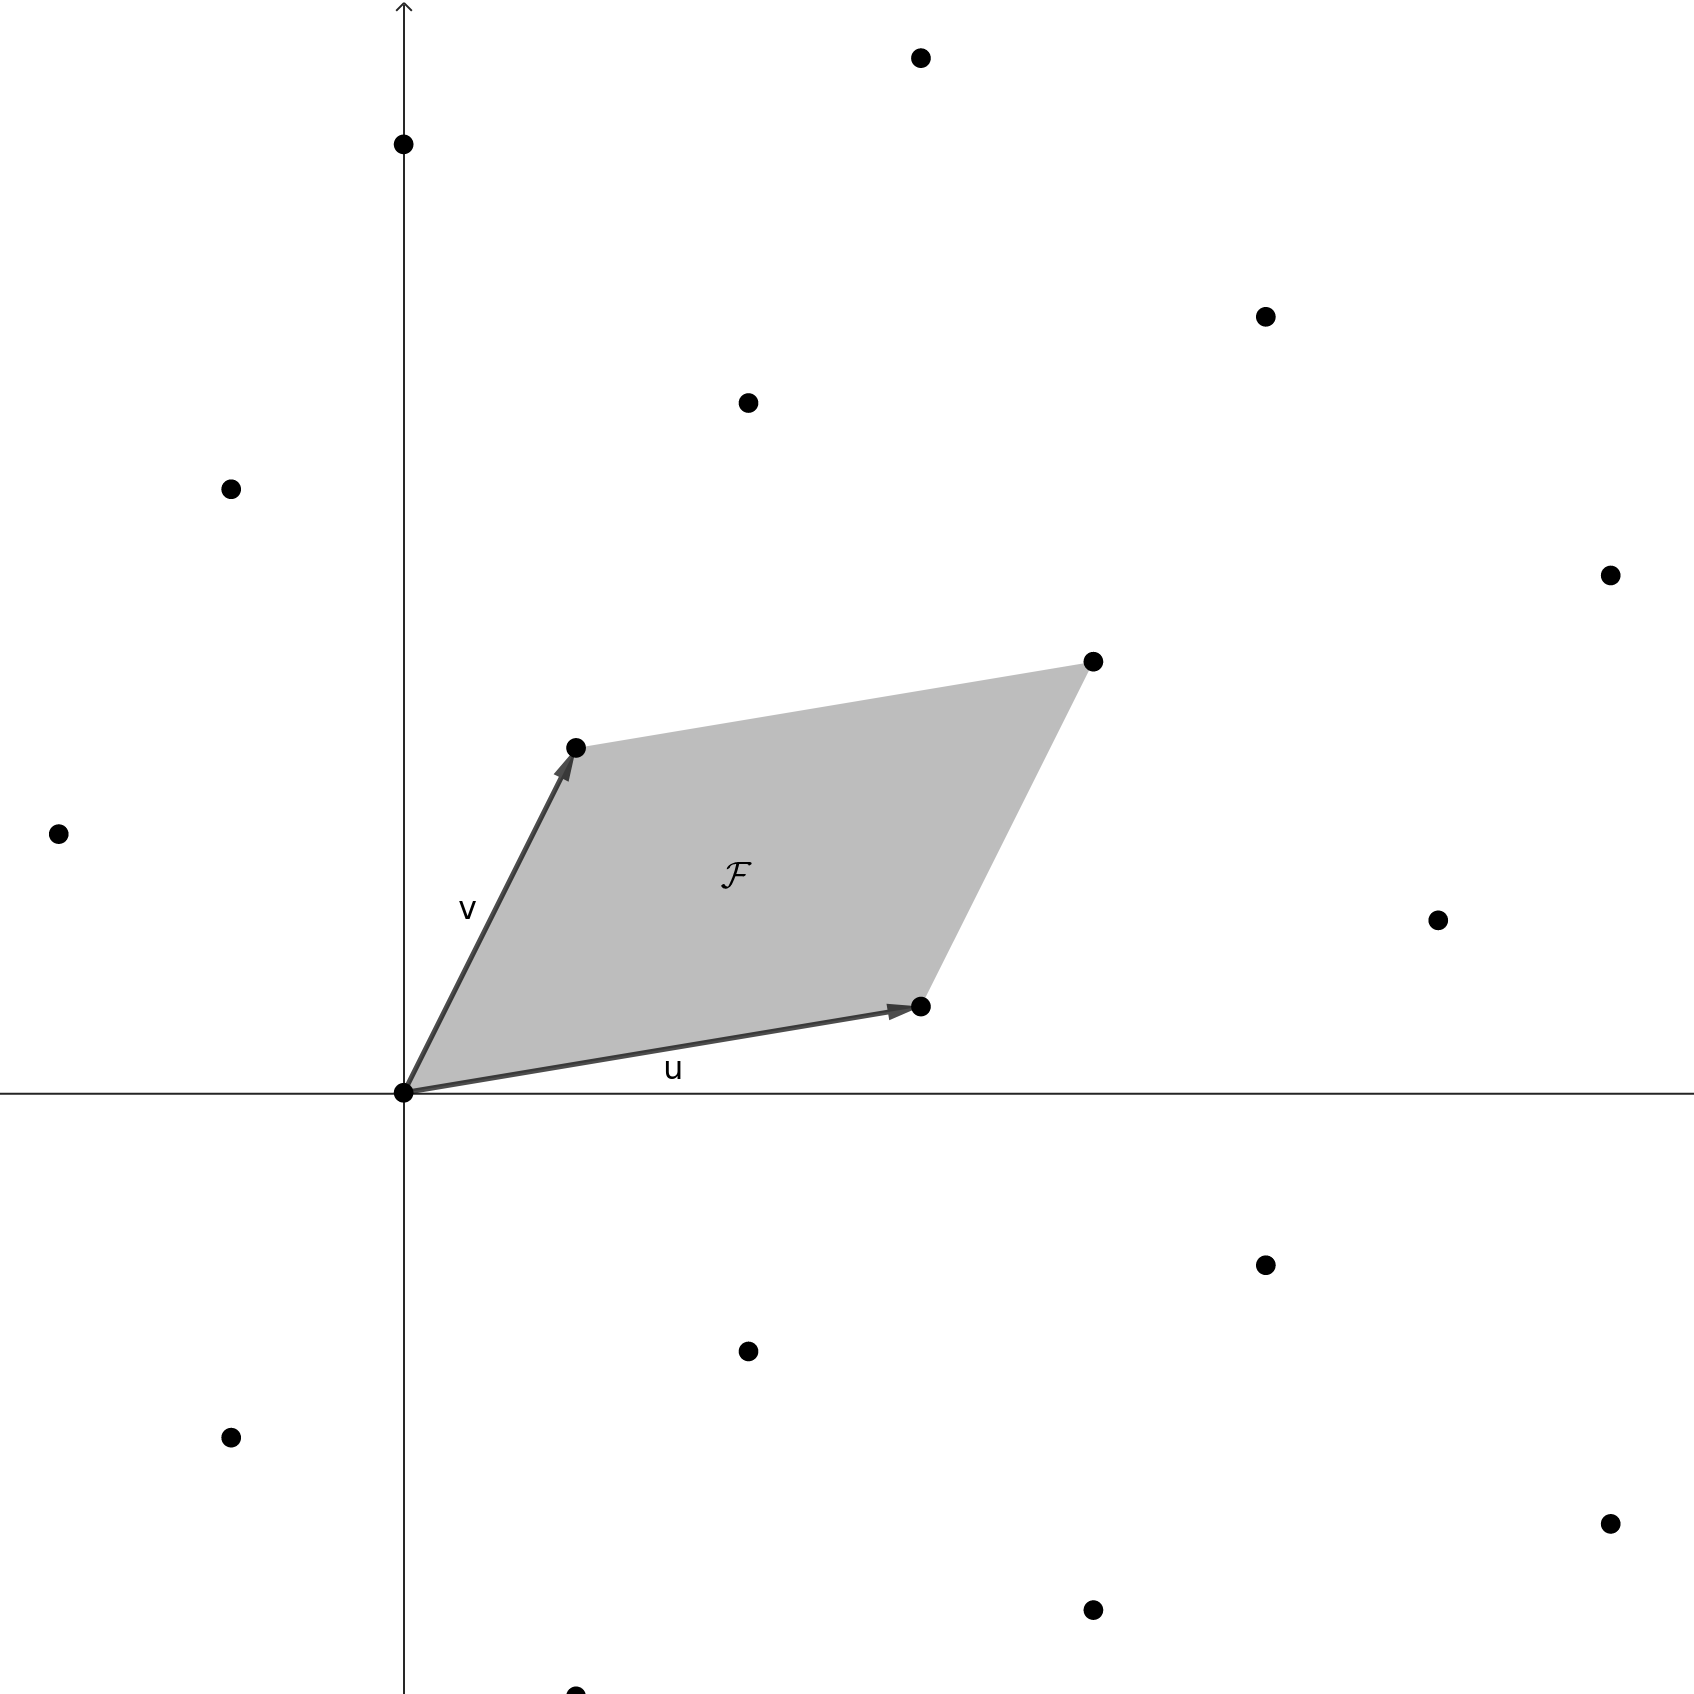
\includegraphics[width=0.75\textwidth]{Figuras/dominio_fundamental.png}\\
        \footnotesize{Fonte: O autor.}
        \label{fig:dominio_fundamental}
    \end{figure}

    As regiões sombreadas da Figura \ref{fig:dominio_fundamental_2} representam os domínios fundamentais de um mesmo reticulado de dimensão 2 gerado por duas bases diferentes, na qual as áreas dos dois paralelepípedos são as mesmas e nenhum elemento do reticulado está no domínio fundamental, com exceção da origem. Isto significa que ambas as bases geram este mesmo reticulado. Esta é uma das propriedades dos domínios fundamentais segundo \cite{daniele-lattices}.

    \begin{figure}[htb!]
        \caption{Exemplo de domínios fundamentais diferentes com mesma área.}
        \begin{minipage}[c]{0.5\linewidth}
            \centering
            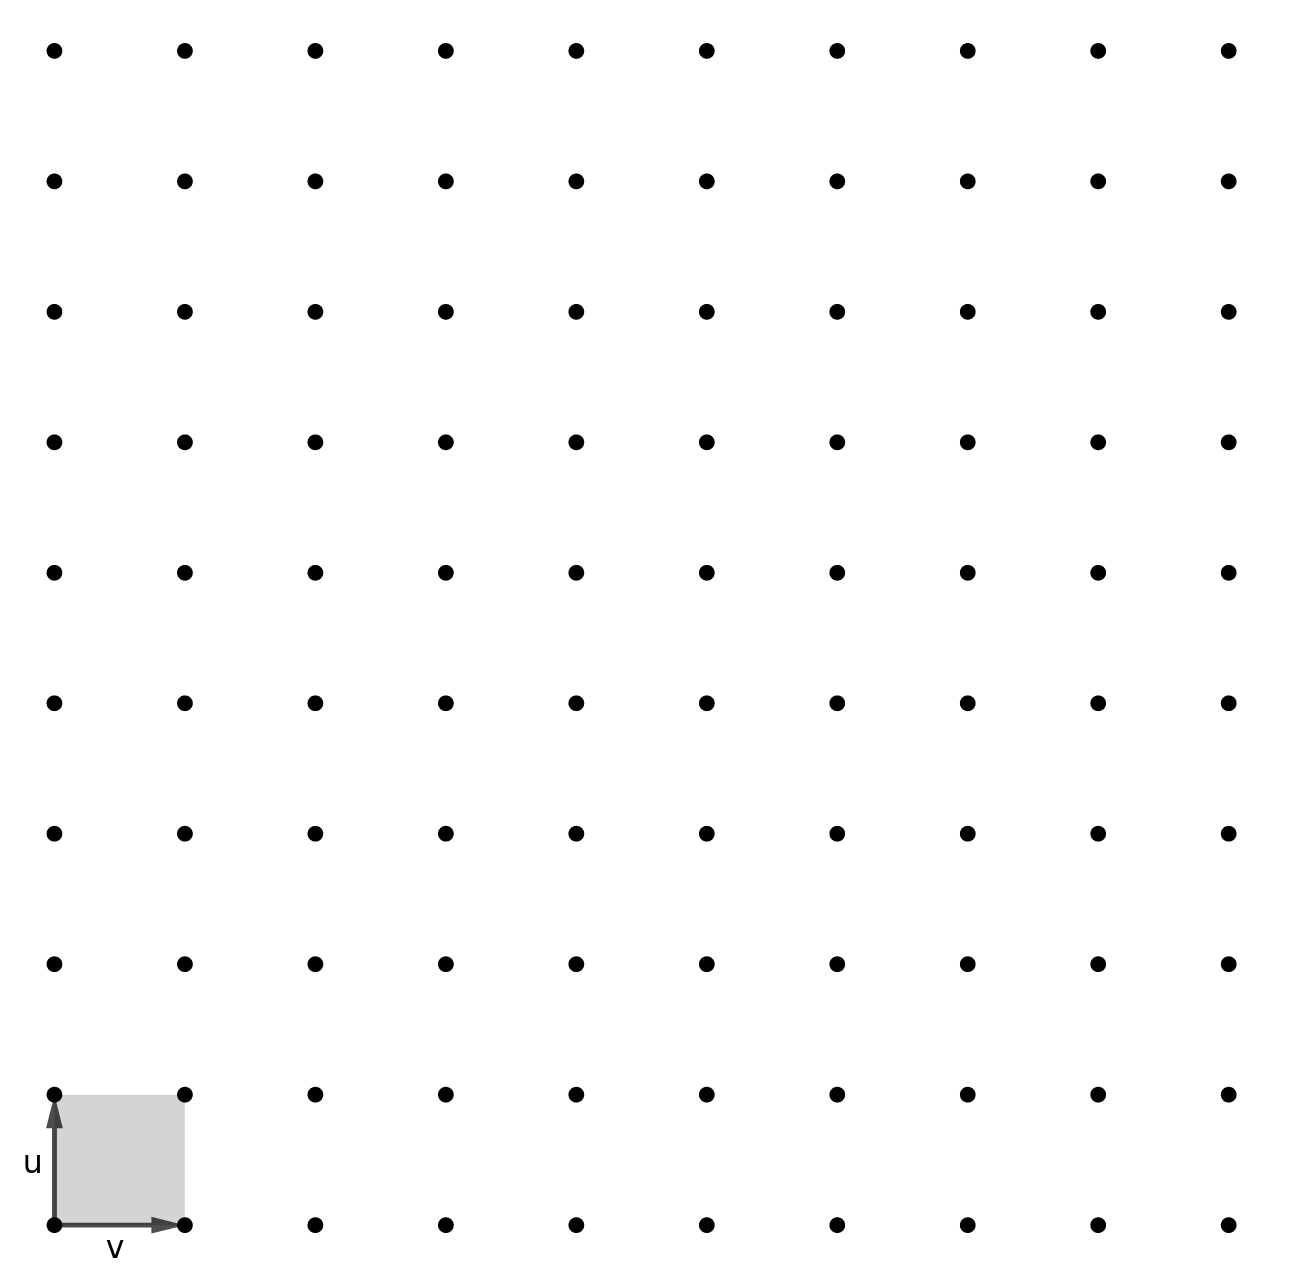
\includegraphics[width=0.75\textwidth]{Figuras/dominio_fundamental_1.png}\\
            \footnotesize{Fonte: O autor.}
        \end{minipage}\hfill
        \begin{minipage}[c]{0.5\linewidth}
            \centering
            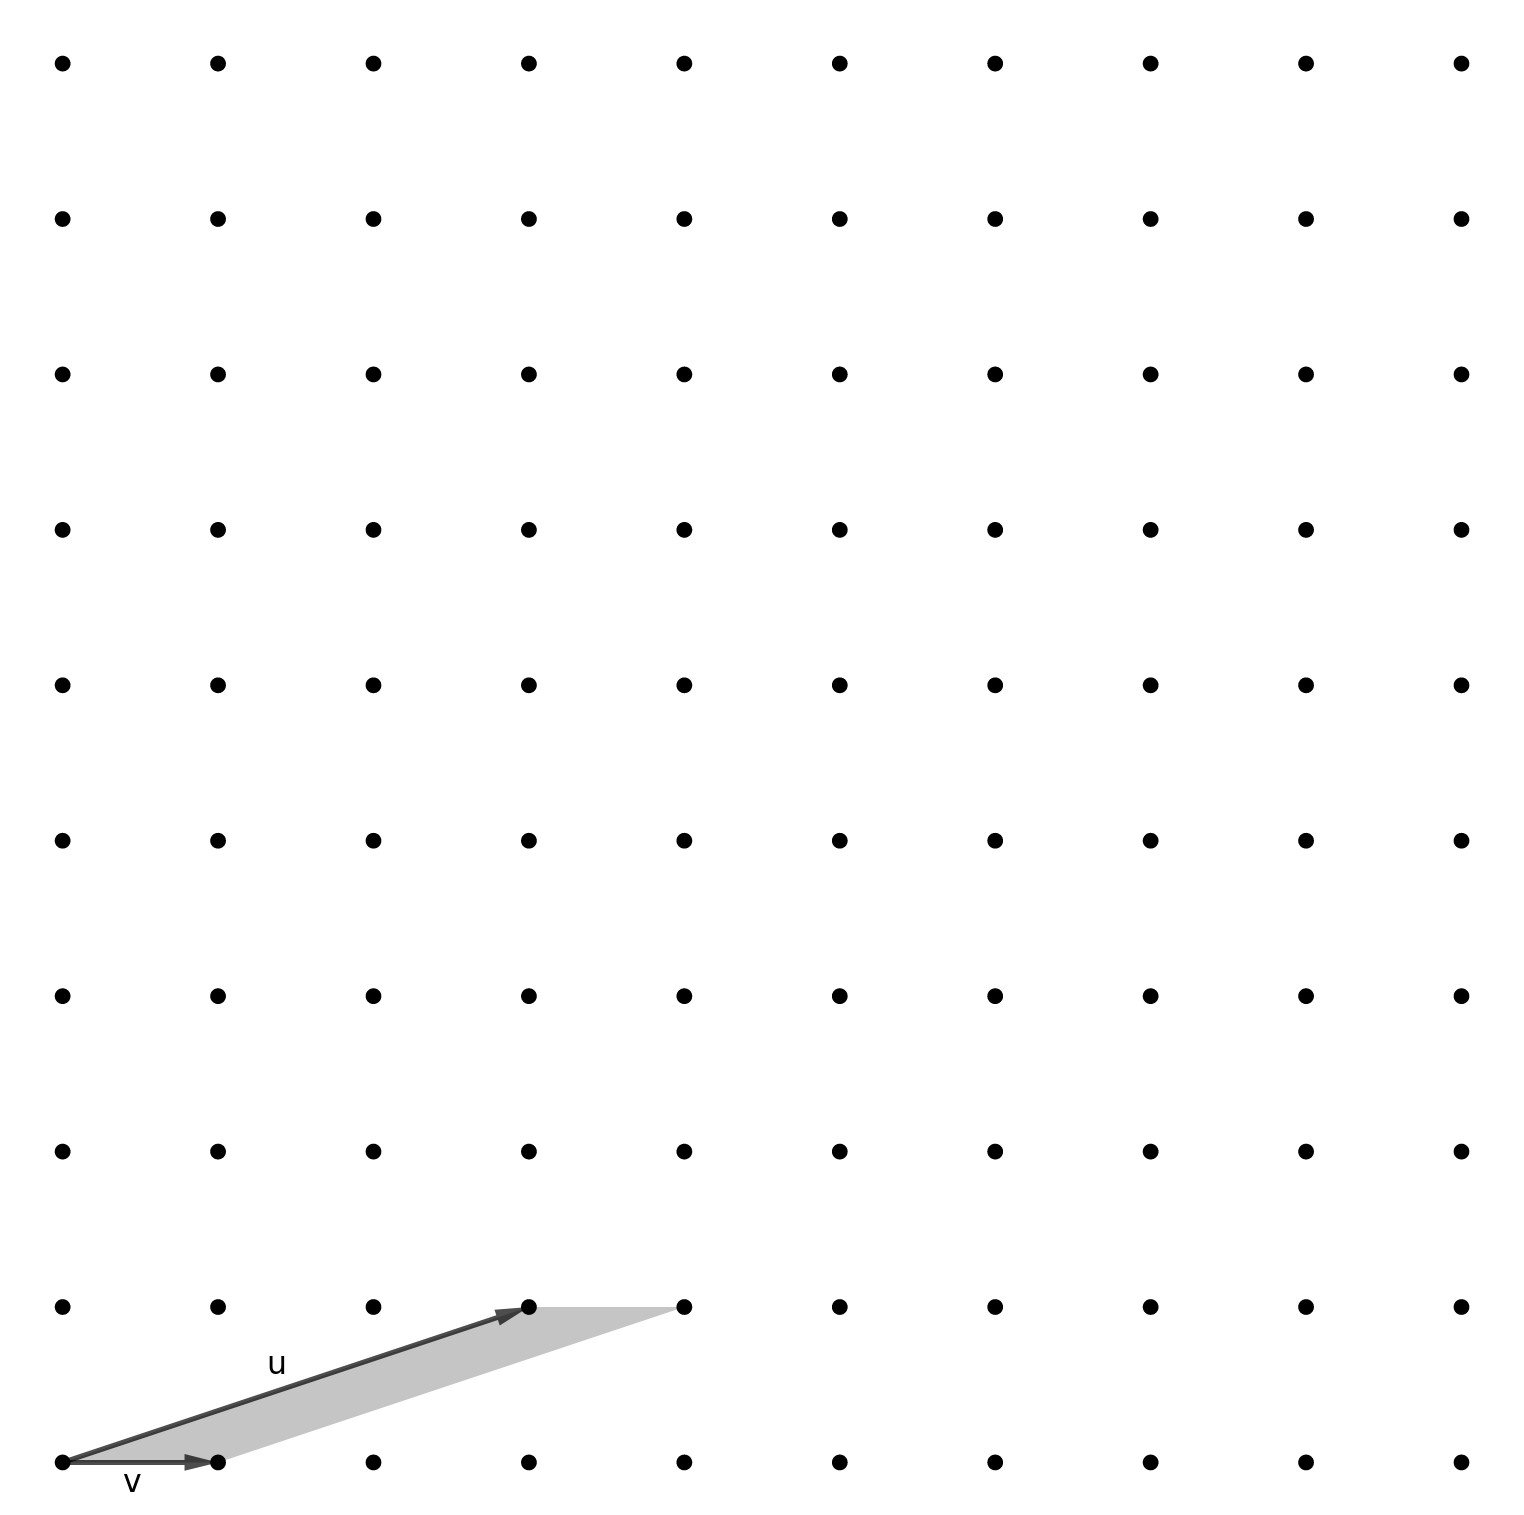
\includegraphics[width=0.75\textwidth]{Figuras/dominio_fundamental_2.png}\\
            \footnotesize{Fonte: O autor.}
        \end{minipage}
        \label{fig:dominio_fundamental_2}
    \end{figure}
    
    Sendo $\mathcal{L}$ um reticulado gerado por uma base $\textbf{B}$, o volume de seu domínio fundamental pode ser calculado pelo valor absoluto da determinante de $\textbf{B}$ na forma matricial, isto é:

    $$Vol(\mathcal{F}_B) = |Det(\textbf{B})|$$

    \noindent
    e também através do algoritmo de Gram Schmidt visto na Seção \ref{cap:reducao_base} por meio da seguinte equação segundo \cite{barros}:

    % = ou <=?
    $$Vol(\mathcal{F}_B) = \prod_{i=1}^{n} \Vert b_{i}^{*} \Vert$$

    \noindent
    em que $B$ é a base de um reticulado de dimensão $n$ e $b_{i}^{*}$ são os vetores gerados pelo algoritmo de Gram Schmidt da base $B$. Embora a base retornada pelo algoritmo de Gram Schmidt não gere o mesmo reticulado da base da entrada, ambas possuem o mesmo volume.

\section{Sucessivas mínimas}
    Seja $B_{n}(0, r) = \{x \in \mathbb{R}^{n}\ |\ ||x|| < r\}$ uma bola de dimensão $n$ centrada na origem e raio $r$. As sucessivas mínimas $\lambda_1, \lambda_2,...,\lambda_n$ de um reticulado $\mathcal{L}$ de dimensão $n$ são constantes, onde $\lambda_i(\mathcal{L})$ é o raio da menor bola de dimensão $i$ centrada na origem que contém $i$ vetores linearmente independentes de $\mathcal{L}$. As sucessivas mínimas de um reticulado $\mathcal{L}(\textbf{B})$  são definidas da seguinte forma:

    $$\lambda_i(\mathcal{L}) = min\{r\ |\ dim(\mathcal{L}(\textbf{B}) \cap \mathcal{B}(0, r)) \geq i  \}$$
    
    Tem-se na Figura \ref{fig:sucessive_minima} um reticulado de duas dimensões, isso significa que este reticulado tem apenas duas sucessivas mínimas $\lambda_1$ e $\lambda_2$. Analisando este reticulado da Figura \ref{fig:sucessive_minima}, a bola de dimensão 1 de menor raio e que contém um vetor linearmente dependente deste reticulado está destacada em uma cor mais escura e possui raio $\lambda_1$, e a bola de dimensão 2 de menor raio que contém os vetores linearmente independentes deste reticulado está destacada em uma cor mais clara e possui raio $\lambda_2$.

    Uma propriedade das sucessivas mínimas é que elas satisfazem $\lambda_1 \leq \lambda_2 \leq\ ...\  \leq \lambda_n$. Desta forma, $\lambda_1$ representa o tamanho do menor vetor de um reticulado com exceção do vetor nulo e também a menor distância entre dois elementos distintos desse reticulado \cite{daniele-lattices}.

    $$\lambda_1(\mathcal{L}) = \min_{x \neq y \in \mathcal{L}} ||x-y|| = \min_{x \in \mathcal{L} - {\vec{0}}} ||x||$$

    Alguns problemas baseados em reticulados estão relacionados com o menor vetor de um reticulado, também denotado por $\lambda_1$.
  
    \begin{figure}[htb!]
        \centering
        \caption{Sucessivas mínimas de um reticulado de duas dimensões.}
        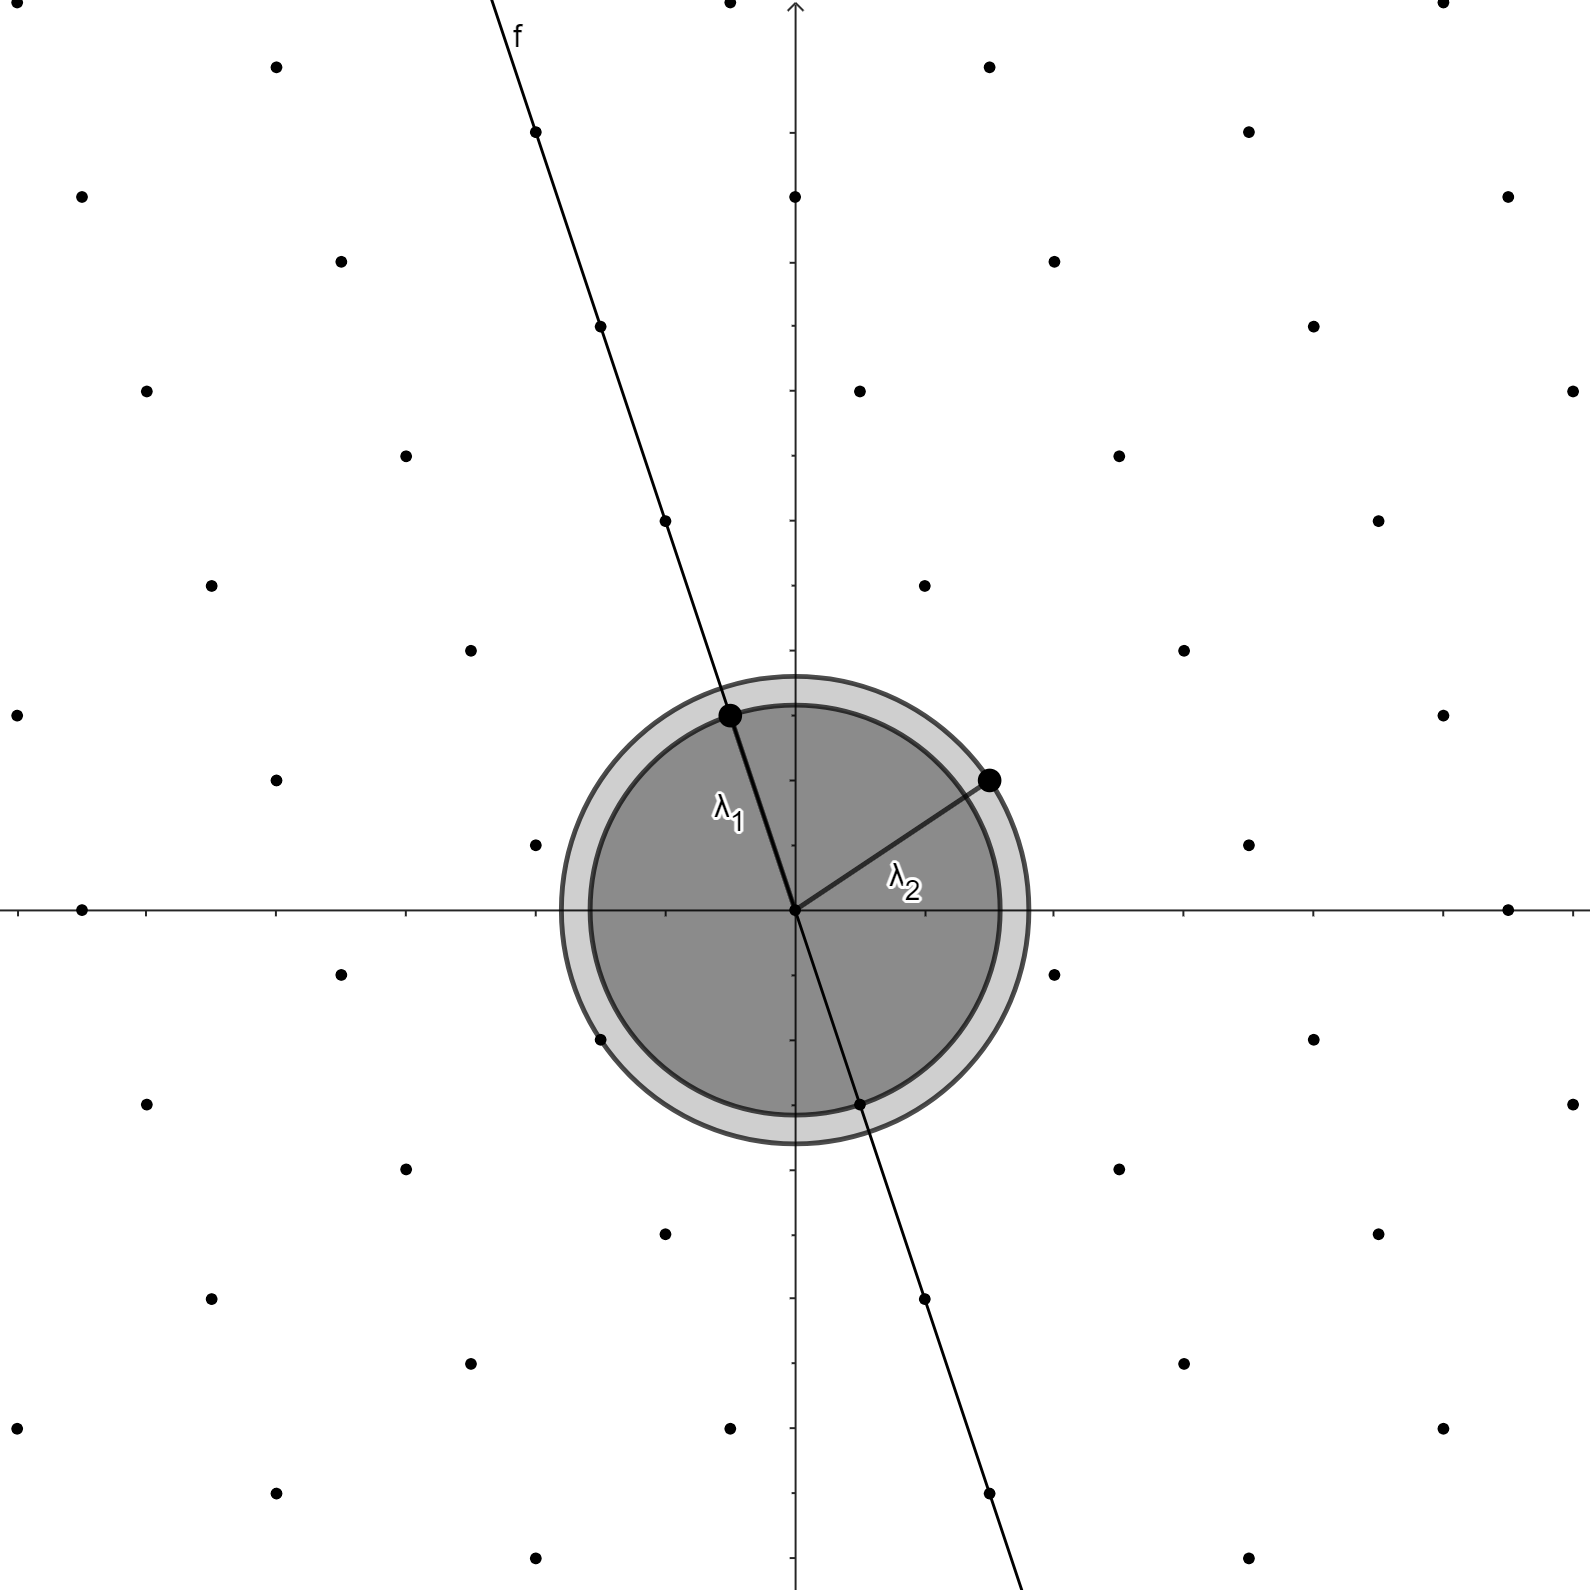
\includegraphics[width=0.75\textwidth]{Figuras/sucessive_minima.png}\\
        \footnotesize{Fonte: O autor.}
        \label{fig:sucessive_minima}
    \end{figure}
    
    As sucessivas mínimas de um reticulado dependem da métrica utilizada. Sejam os vetores $\vec{b_1} = \{2,0\}$ e $\vec{b_2} = \{1,1\}$, usando a métrica $l_1$ definida na Seção \ref{sec:espacos_metricos}, $\lambda_1 = \vec{b_1}$, visto que a norma de $\vec{b_1}$ sob a métrica $l_1$ é $2$. Entretanto, $\lambda_1 \neq \vec{b_1}$ se utilizadas as normas $l_2$ ou $l_{\infty}$ por exemplo. Isso se dá devido a $\vec{b_2}$ ser menor que $\vec{b_1}$ quando usadas essas métricas \cite{daniele-lattices}. Dessa forma, ao realizar uma análise de um problema computacional envolvendo sucessivas mínimas, deve-se ter bem definida qual métrica está sendo utilizada.

\section{Problemas computacionais}
\label{cap:lattice_problems}

%https://www.youtube.com/watch?v=o4Pl-0Q5-q0&ab_channel=SimonsInstitute -> EXPLICA MÉTODO SIEVING
%https://www.youtube.com/watch?v=LzWjLGG9cJI&ab_channel=TanjaLange%3APost-quantumcryptography -> EXPLICA MÉTODO ENUMERATION
%https://iacr.org/archive/crypto2007/46220170/46220170.pdf ->ENUMERATION
%https://math.mit.edu/~apost/courses/18.204-2016/18.204_Xinyue_Deng_final_paper.pdf -> LLL

%############################### TEM TUDO AQUIII #####################################
%#                    https://eprint.iacr.org/2012/533.pdf                           #
%#####################################################################################

%##################### IMPORTANTE PARA DEFIRNIR MODULAR LATTICES
%for any lattice B and point x ∈ span(B), there exists a unique vector y ∈ P(B) such that y − x ∈ L(B). This vector is denoted y = x mod B ->https://ieeexplore.ieee.org/document/1366257 

    
    Nesta seção serão apresentados alguns dos principais problemas computacionais sobre a estrutura de reticulados que formam a base da segurança dos sistemas de criptografia que utilizam esta estrutura. Como será visto nas Seções \ref{cap:algoritmos_exatos} e \ref{cap:reducao_base}, os algoritmos que resolvem estes problemas possuem complexidade exponencial ou pior, e os que executam em tempo polinomial conseguem apenas aproximações distantes do resultado ótimo para reticulados com certas propriedades, como dimensão, ortogonalidade e tamanho da norma dos vetores que formam a base do reticulado. Devido a este fato, os algoritmos que se baseiam nesses problemas são considerados seguros. 

    %https://dl.acm.org/doi/pdf/10.1145/237814.237838
    %The Complexity of Some Lattice Problems Jin-Yi Cai*
    %The Hardness of Approximate Optima in Lattices, Codes, and Systems of Linear Equations
    %danielle maciamicio
    
    \begin{definition}[\textit{Closest Vector Problem} (CVP)]
        O problema \ac{CVP} consiste em, dado um reticulado $\mathcal{L}$ e um vetor $\vec{c} \notin \mathcal{L}$, encontrar um vetor $\vec{v} \in \mathcal{L}$ tal que a distância entre $\vec{c}$ e $\vec{v}$ seja mínima.
    \end{definition}

    Intuitivamente, o problema \ac{CVP} pode ser aplicado à criptografia da seguinte maneira, seja $\vec{v} \in \mathcal{L(\beta)}$ uma chave privada, é somado a esta chave um vetor aleatório $\vec{e} \notin \mathcal{L(\beta)}$ com norma pequena, o resultado dessa soma é uma chave pública $\vec{c} \notin \mathcal{L(\beta)}$, dessa forma, para se recuperar a chave privada é preciso encontrar o vetor mais próximo de $\vec{c}$, que nesse caso seria a chave privada $\vec{v}$. Este é um dos principais problemas envolvendo reticulados e foi demonstrado por \cite{np-hard-cvp-svp} pertencer à classe dos problemas \ac{NP-HARD} para todas as normas $l_p$. A Figura \ref{fig:cvp} ilustra o problema \ac{CVP} em um reticulado de duas dimensões.
    
    \begin{definition}[\textit{Shortest Vector Problem} (SVP)]
         O problema \ac{SVP} consiste em, dado um reticulado $\mathcal{L}$, encontrar um vetor $\vec{v} \in \mathcal{L}$ tal que $\lVert \vec{v} \rVert$ seja mínima.
    \end{definition}

    Outro problema importante associado a reticulados é o problema \ac{SVP}, diferente do problema \ac{CVP}, este consiste em encontrar o vetor mais próximo da origem, que seria no caso o menor vetor do reticulado. Devido a essa relação com o problema \ac{CVP}, existe uma redução do problema \ac{SVP} para o \ac{CVP}, demonstrada em \cite{svp_to_cvp}. O problema \ac{SVP} foi demonstrado pertencer à classe \ac{NP-HARD} para a métrica $l_{\infty}$ por \cite{np-hard-cvp-svp}. A Figura \ref{fig:svp} ilustra este problema, em que $w$ é o vetor mais curto do reticulado.

    \begin{figure}[htb!]
        \begin{minipage}[c]{0.5\linewidth}
            \centering
            \caption{Ilustração do problema CVP.}
            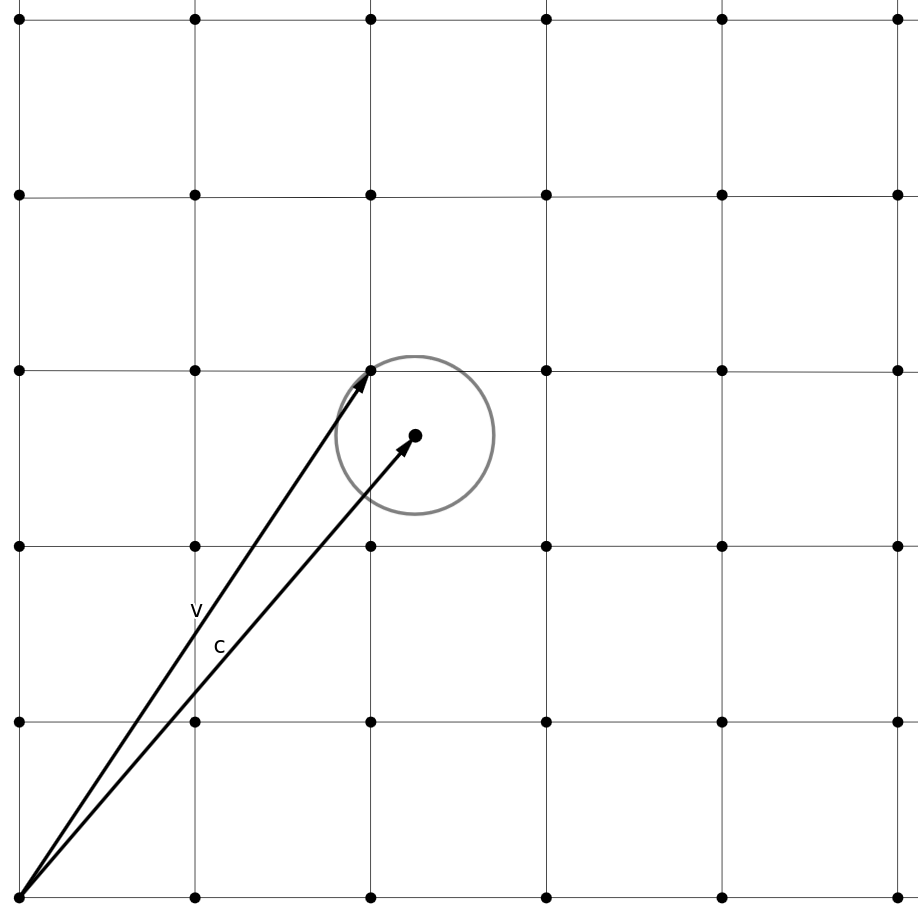
\includegraphics[width=0.75\textwidth]{Figuras/cvp.png}\\
            \footnotesize{Fonte: O autor.}
            \label{fig:cvp}
        \end{minipage}\hfill
        \begin{minipage}[c]{0.5\linewidth}
            \centering
            \caption{Ilustração do problema SVP.}
            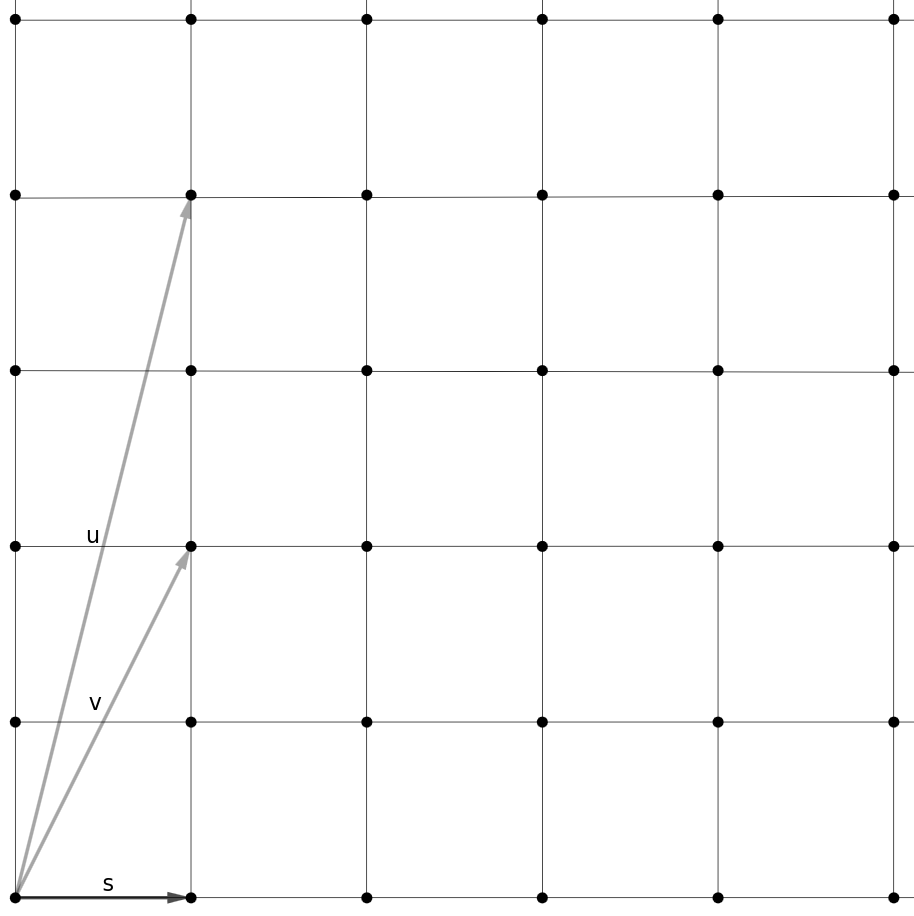
\includegraphics[width=0.75\textwidth]{Figuras/svp.png}\\
            \footnotesize{Fonte: O autor.}
            \label{fig:svp}
        \end{minipage}
    \end{figure}
    
    \begin{definition}[$CVP_\gamma$]
        O problema $CVP_\gamma$ consiste em dado um reticulado $\mathcal{L}$, um vetor $\vec{c} \notin \mathcal{L}$ e um fator de aproximação $\gamma \ge 1$, encontrar um vetor $v \in \mathcal{L}$ tal que $\|\vec{c} - \vec{v}\| \le \gamma d(\vec{c}, \mathcal{L})$.
    \end{definition}

    \begin{definition}[$SVP_\gamma$]
         O problema $SVP_\gamma$ consiste em, dado um reticulado $\mathcal{L}$ e um fator de aproximação $\gamma \ge 1$, encontrar um vetor $\vec{v} \in \mathcal{L}$ tal que $0 < \lVert \vec{v} \rVert \le \gamma \lambda_{1}(\mathcal{L})$. 
    \end{definition}

    Os problemas que utilizam um fator de aproximação, como $CVP_\gamma$ e $SVP_\gamma$, são estudados nos algoritmos que conseguem apenas uma aproximação do resultado ótimo para estes problemas. Esse fator geralmente está em função do grau do reticulado, por exemplo $\gamma(n) = (2 / \sqrt{3})^n$, isso significa que o resultado desse algoritmo estará no máximo a $\gamma$ de distância do resultado ótimo. Os algoritmos que resolvem uma aproximação desses problemas se encontram na Seção \ref{cap:reducao_base}.

     \begin{definition}[\textit{Gap Shortest Vector Problem} ($GapSVP_\gamma$)]
        O problema $GapSVP_\gamma$ consiste em, dado um reticulado $\mathcal{L}$ e um número real positivo $d$, determinar se $\lambda_1(\mathcal{L}) \leq d$ ou $\lambda_1(\mathcal{L}) > \gamma d$.
    \end{definition}

    \begin{definition}[\textit{Shortest Independent Vector Problem} ($SIVP_\gamma$)]
        O problema $SIVP_\gamma$ consiste em, fornecido um reticulado $\mathcal{L}$ de dimensão $n$, encontrar um conjunto de $n$ vetores linearmente independentes com comprimento máximo de $\gamma \lambda_{n}(\mathcal{L})$.
    \end{definition}
    
    \begin{definition}[\textit{Learning With Errors} (LWE)]
        Dado uma matriz $\textbf{A} \in \mathbb{Z}_p^{m \times n}$ gerada por uma distribuição de probabilidade uniforme e uma matriz $\textbf{t} = \textbf{As} + \textbf{e} \in \mathbb{Z}_p^m$, sendo $\textbf{e} \in \mathbb{Z}_p^m$ um erro adicional especificado por uma distribuição de probabilidade $\chi:\mathbb{Z}_p \to \mathbb{R}^{+}$ em $\mathbb{Z}_p$, encontrar a matriz $\textbf{s} \in \mathbb{Z}_p^n$ \cite{regev}. 
    \end{definition}

    \begin{figure}[htb!]
        \centering
        \caption{Ilustração do problema \ac{LWE}.}
        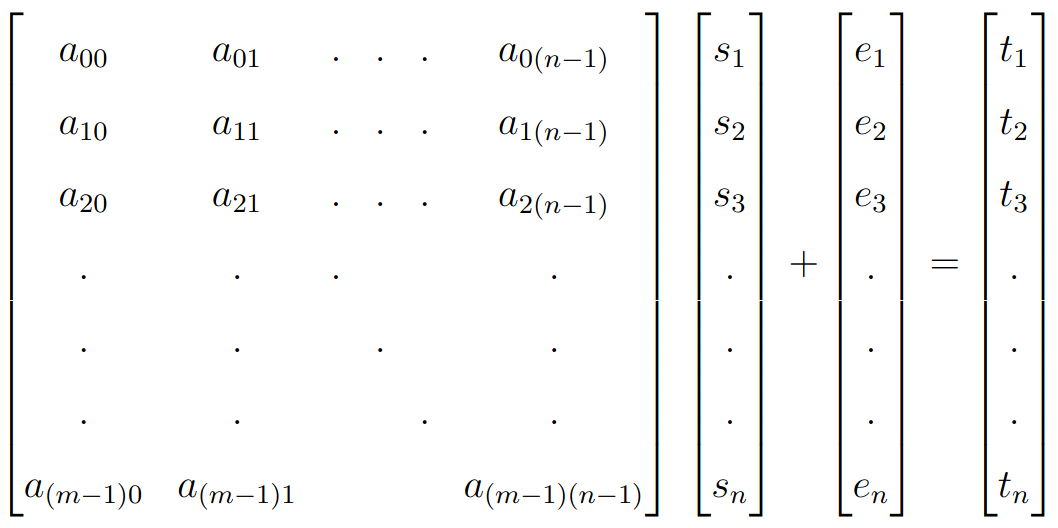
\includegraphics[width=0.65\textwidth]{Figuras/lwe.png}\\
        \footnotesize{Fonte: O autor.}
        \label{fig:lwe}
    \end{figure}

    O problema \ac{LWE} foi introduzido por \cite{regev} e consiste na dificuldade de se obter a solução para uma equação linear com um erro, como pode ser observado na Figura \ref{fig:lwe}. Perceba que sem a matriz de erro/ruído \textbf{e}, este problema poderia ser facilmente resolvida pela eliminação Gaussiana em tempo $\mathcal{O}(n)$, sendo $n$ o número de equações a serem resolvidas. Entretanto, se adicionarmos um erro aleatório a essa equação, resolvê-la é uma tarefa difícil, até para computadores quânticos. O artigo \cite{regev} relata a dificuldade de se encontrar algoritmos clássicos e quânticos que resolvem este problema em tempo polinomial, o que o torna útil para a criação de sistemas de criptografia baseados neste problema. A complexidade de resolução do \ac{LWE} está relacionada com a dificuldade de resolução dos problemas \ac{GapSVP} e \ac{SIVP}, visto que \cite{regev} demonstra uma redução destes problemas para \ac{LWE}.

    Este problema, além de ser seguro contra computadores quânticos, chamou atenção devido a sua versatilidade, eficiência e simplicidade. Ele foi a base para a criação de outros problemas computacionais como \ac{RLWE}, \ac{MLWE} e também outros modelos de criptografia, como criptografia homomórfica.

    Um aspecto a ser considerado ao utilizar o \ac{LWE} é o tamanho da chave pública, representado pela matriz \textbf{A}. Em que a complexidade de espaço é $\mathcal{O}(n^2)$, sendo $n$ a ordem da matriz \textbf{A}. Esta é uma das razões pela qual este problema não é utilizado na prática em sistemas criptográficos. O problema \textit{Ring Learning With Errors} (RLWE) apresenta uma alternativa para diminuir o tamanho da matriz \textbf{A} e melhorar o desempenho das operações de multiplicação matricial devido à seguinte relação:

        \begin{center}
            $\begin{bmatrix}
                b_{1}   & -b_{n}   & -b_{n-1} & . & . & . & -b_{2}\\
                b_{2}   &  b_{1}   & -b_{n-2} & . & . & . & -b_{3}\\
                b_{3}   &  b_{2}   &  b_{1}   & . & . & . & -b_{4}\\
                .       & .        &          & . & . & . & .     \\
                .       & .        &          &   & . & . & .     \\
                .       & .        &          &   &   & . & .     \\
                b_{n} & b_{n-1}&              &   &   &   & b_{1}
            \end{bmatrix}$
            %
            $\begin{bmatrix}
                s_1  \\
                s_2  \\
                s_3  \\
                .    \\
                .    \\
                .    \\
                s_{n}
            \end{bmatrix}$
            %
            $\Leftrightarrow$
            %
            $(b_1 + b_2 x + b_3 x^2 + ... + b_{n} x^{n-1})(s_1 + s_2 x + s_3 x^2 + ... + s_{n} x^{n-1})\ \textbf{mod}\ x^n + 1$
        \end{center}
    
    Dessa forma é possível obter os demais elementos da matriz a partir da primeira coluna, sendo assim, necessário apenas armazenar a primeira coluna, o que resulta em uma diminuição do tamanho da chave criptográfica. 
    
    \begin{definition}[\textit{Ring Learning With Errors} (RLWE)]
        Seja $A \in \mathbb{Z}_q{[}x{]} / \langle x^n+1 \rangle$ gerada por uma distribuição de probabilidade uniforme e um polinômio $t = As + e \in \mathbb{Z}_q{[}x{]} / \langle x^n+1 \rangle$ sendo $e \in \mathbb{Z}{[}x{]} / \langle x^n+1 \rangle$ especificado por uma distribuição de probabilidade $\chi$ em $\mathbb{Z}{[}x{]} / \langle x^n+1 \rangle$ com desvio padrão $\sigma$, considerando-o em $\mathbb{Z}_q{[}x{]} / \langle x^n+1 \rangle$, encontrar o polinômio $s \in \mathbb{Z}_q{[}x{]} / \langle x^n+1 \rangle$ \cite{ring_lwe}. 
    \end{definition}
    
    A redução do tamanho da chave não é a única vantagem oferecida pelo \ac{RLWE}, transformando os vetores $\vec{b}$ e $\vec{s}$ em polinômios através do isomorfismo $\sigma_1:P[x] \to \mathbb{Z}^n$, a multiplicação entre $\sigma_{1}^{-1}(\vec{b})$ e $\sigma_{1}^{-1}(\vec{s})$ módulo $x^n + 1$ é equivalente à multiplicação matricial acima. A realização de uma operação de multiplicação polinomial modular, em vez da matricial, proporciona aceleração à operação de multiplicação por meio do algoritmo \ac{NTT} \cite{ntt}, onde a complexidade passa a ser $\mathcal{O}(n log(n))$. A redução do tamanho da chave, segundo \cite{ring_lwe}, não reduz a complexidade do problema, desde que se escolha os parâmetros $\sigma$, $n$ e $q$ adequadamente.
    
    \begin{definition}[\textit{Module Learning With Errors} (MLWE)]
        Seja $\textbf{A} \in {[}\mathbb{Z}_q{[}x{]} / \langle x^n+1 \rangle{]}^{m \times k}$ gerada por uma distribuição de probabilidade uniforme e uma matriz $\textbf{t} = \textbf{As} + \textbf{e} \in {[}\mathbb{Z}_q{[}x{]} / \langle x^n+1 \rangle{]}^{m}$ sendo $\textbf{e} \in {[}\mathbb{Z}_q{[}x{]} / \langle x^n+1 \rangle{]}^{m}$, encontrar a matriz $\textbf{s} \in {[}\mathbb{Z}_q{[}x{]} / \langle x^n+1 \rangle{]}^{k}$ \cite{module-lwe}. 
    \end{definition}

    \begin{figure}[htb!]
        \centering
        \caption{Ilustração do problema \ac{MLWE}.}
        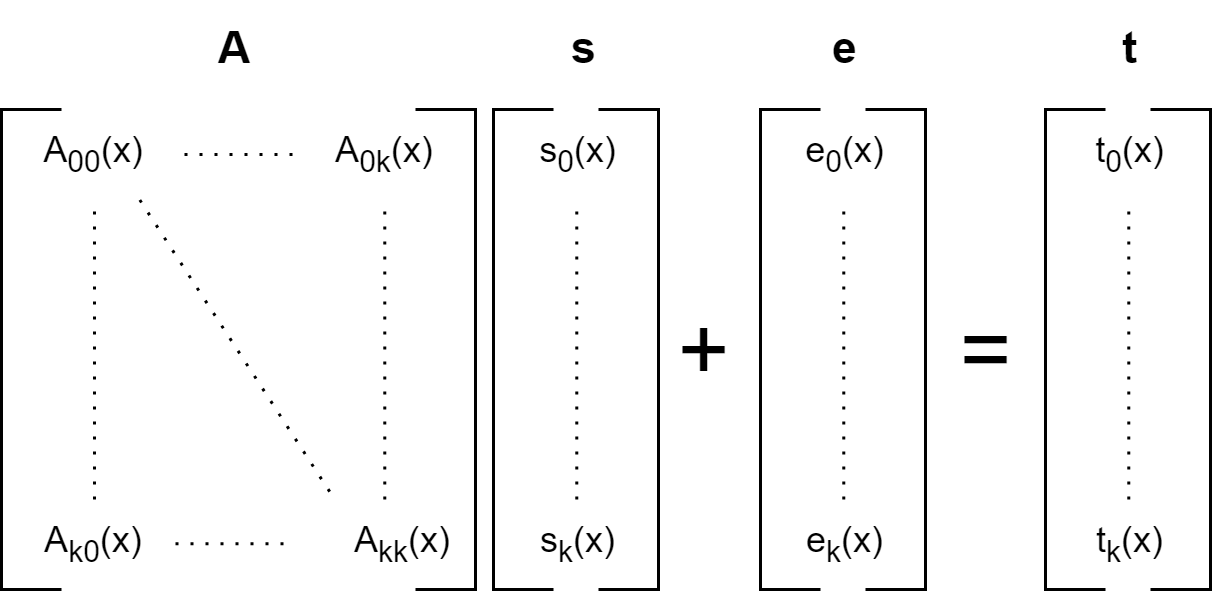
\includegraphics[width=0.75\textwidth]{Figuras/kyber_keygen.png}\\
        \footnotesize{Fonte: O autor.}
        \label{fig:mlwe}
    \end{figure}

    O problema \ac{MLWE} é semelhante ao problema \ac{LWE} como pode ser observado na Figura \ref{fig:mlwe}, com a diferença que os elementos das matrizes, em vez de inteiros, agora são polinômios. O \ac{MLWE} pode ser interpretado como vários problemas \ac{RLWE} dentro do \ac{LWE}, visto que se alterado o parâmetro $k$ para 1, tem-se exatamente o problema \ac{RLWE}. Segundo a documentação oficial do \ac{ML-KEM} \cite{kyber}, os autores optaram por utilizar o \ac{MLWE} por preocupações que a estrutura \ac{RLWE} possa permitir ataques mais eficientes, além de que o \ac{MLWE} possui uma melhor escalabilidade e eficiência semelhante ao \ac{RLWE} para determinados parâmetros \cite{kyber2}.

\section{Algoritmos exatos}
\label{cap:algoritmos_exatos}
    Existem duas técnicas que resolvem com exatidão os problemas SVP e CVP, a técnica de \textit{sieving} e a técnica de \textit{enumeration}. 
    
    A técnica de \textit{sieving} foi proposta pela primeira vez em 2001 por Miklós Ajtai, Ravi Kumar e D. Sivakumar \cite{sieving}, e existem diversas variações deste algoritmo com complexidade de tempo inferior ao algoritmo original $\mathcal{O}(2^n)$, porém ainda com complexidade exponencial de tempo e espaço, o que torna estes algoritmos impraticáveis para reticulados de grandes dimensões. A ideia principal desta técnica é selecionar um conjunto de vetores em uma região de raio $R$ de um reticulado, realizar sucessivas subtrações entre pares de vetores deste conjunto e adicionar os vetores resultantes dessas operações ao conjunto final caso sua norma for menor que $\gamma R$ para $0< \gamma < 1$. A Figura \ref{fig:sieving} ilustra a ideia-chave dos algoritmos que utilizam a técnica de \textit{sieving}. 

    \begin{figure}[htb!]
        \centering
        \caption{Exemplo do funcionamento do algoritmo \textit{sieving} com duas iterações respectivamente.}
            \begin{subfigure}{.5\textwidth}
                \centering
                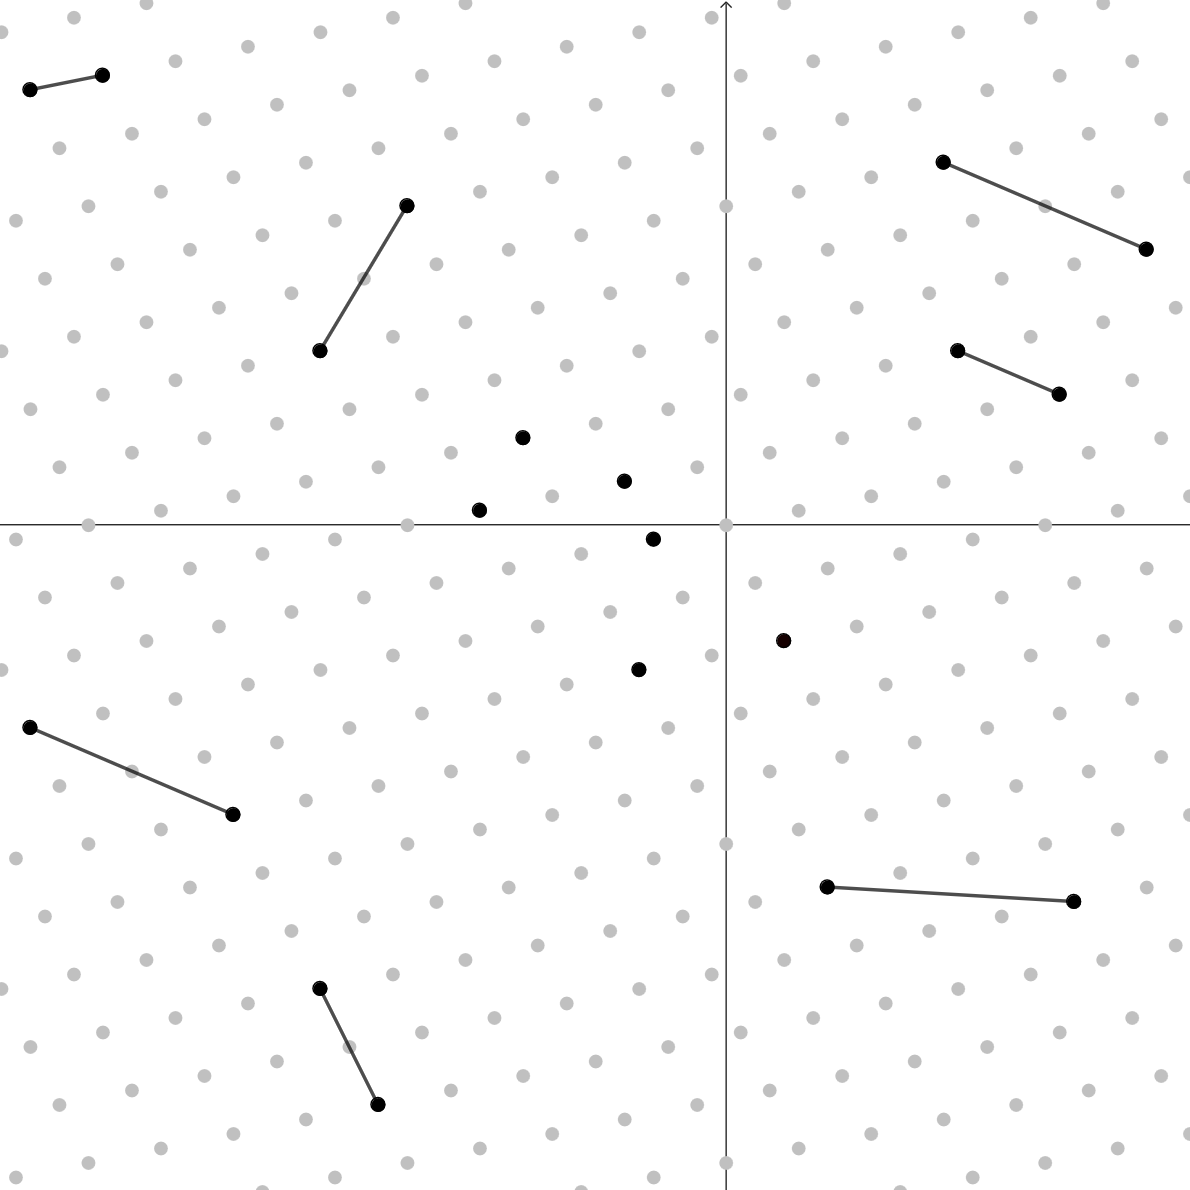
\includegraphics[width=.75\linewidth]{Figuras/sieving_1.png}
            \end{subfigure}%
            \begin{subfigure}{.5\textwidth}
                \centering
                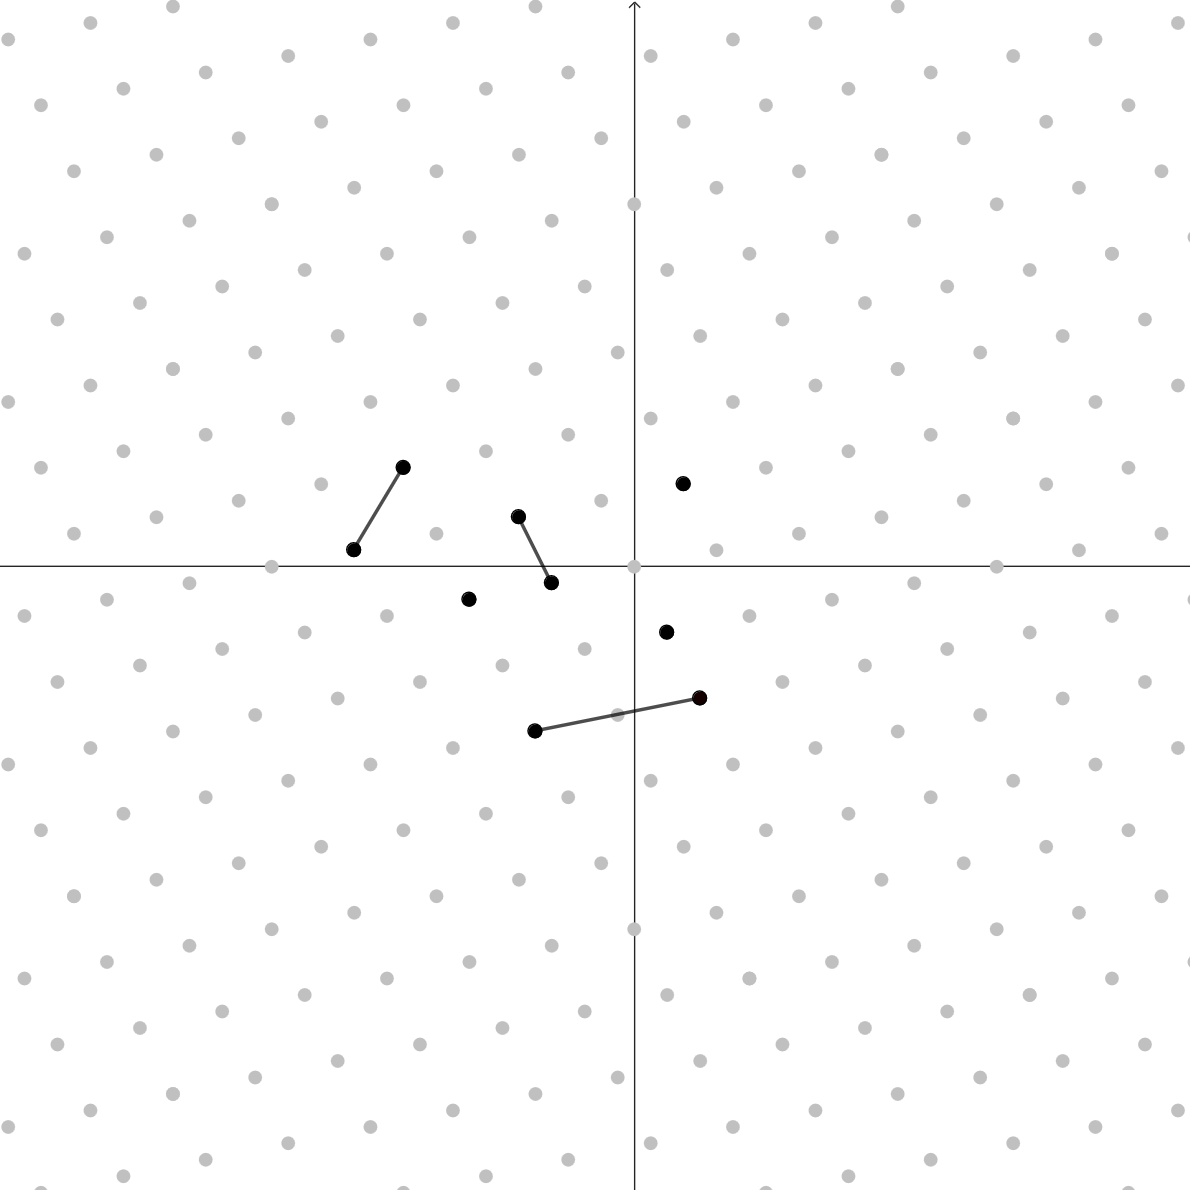
\includegraphics[width=.75\linewidth]{Figuras/sieving_2.png}
            \end{subfigure}
        \footnotesize{Fonte: O autor.}
        \label{fig:sieving}
    \end{figure}

    %https://sci-hub.se/http://dx.doi.org/10.1090/S0025-5718-1985-0777278-8
    A técnica de \textit{enumeration} foi proposta pela primeira vez por U. Fincke e M. Pohst em 1985 \cite{enumeration_fincke_pohst}, entretanto, devido à sua complexidade de $\mathcal{O}(2^{n^2})$, é mais conhecido o algoritmo proposto por Ravi Kannan de 1987, com complexidade de $\mathcal{O}(n^n)$ \cite{enumeration_kannan}. Este algoritmo, assim como o AKS, também resolve o problema SVP com exatidão, e embora possua complexidade de tempo maior que o algoritmo AKS $\mathcal{O}(n^n)$, este algoritmo tem a vantagem de possuir complexidade polinomial de espaço. A ideia principal dos algoritmos de \textit{enumeration} é selecionar duas bases $\vec{b_1}$ e $\vec{b_2}$, calcular a projeção de $\vec{b_2}$ sobre a reta ortogonal a $\vec{b_1}$. O próximo passo é enumerar os vetores em uma região que estão a uma distância múltipla da norma do vetor resultante da projeção de $\vec{b_2}$ sobre a reta ortogonal a $\vec{b_1}$. A partir destes vetores enumerados o algoritmo de Kannan encontra o vetor mais curto nesta região. A Figura \ref{fig:lattice_enumeration} ilustra este processo, onde os pontos destacados são os vetores enumerados pelo algoritmo.

    \begin{figure}[htb!]
        \centering
        \caption{Exemplo do funcionamento do algoritmo \textit{enumeration}.}
        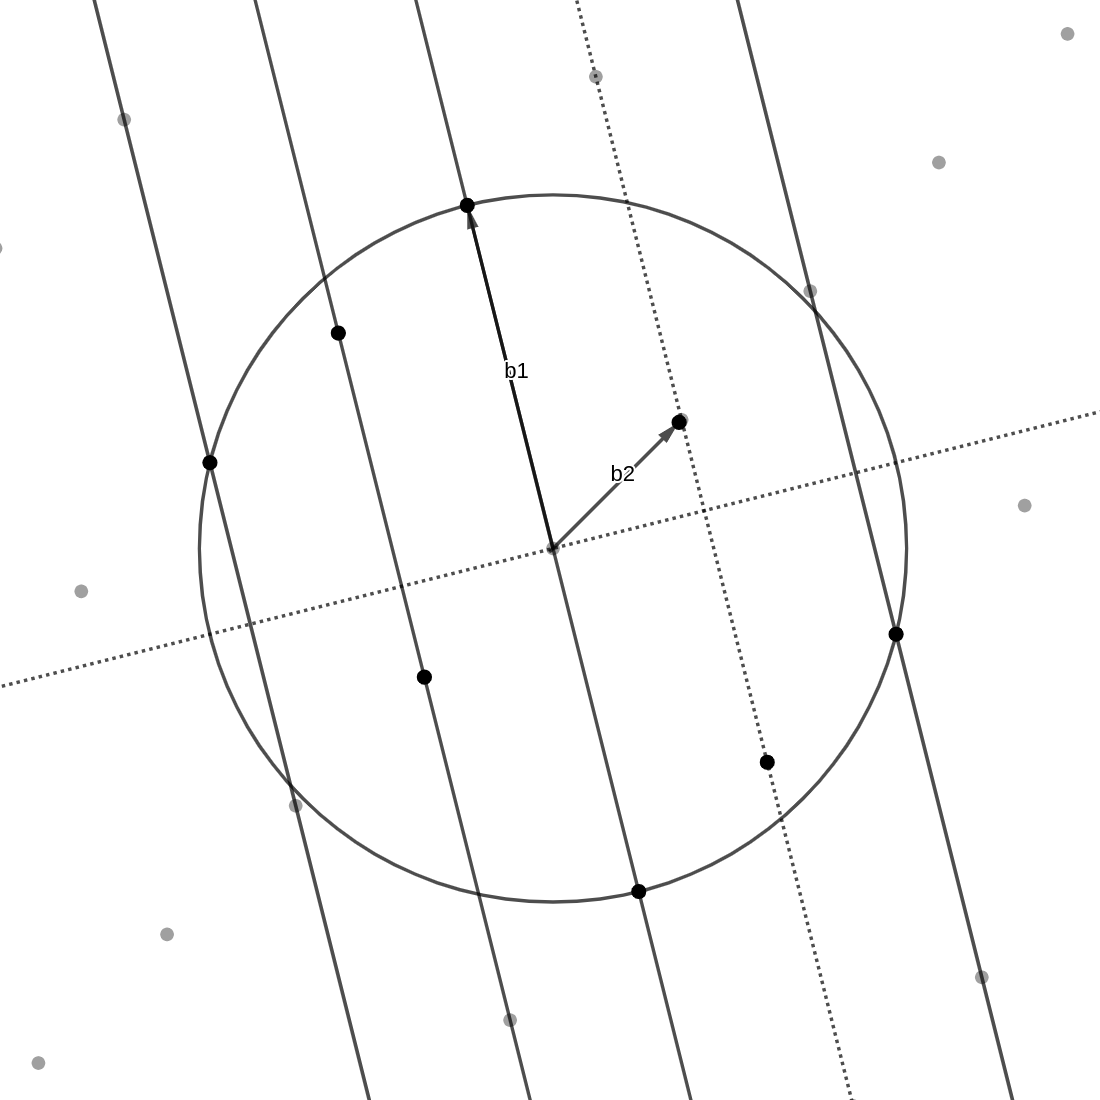
\includegraphics[width=0.65\textwidth]{Figuras/lattice_enumeration.png}\\
        \footnotesize{Fonte: O autor.}
        \label{fig:lattice_enumeration}
    \end{figure}

\section{Redução de base}
\label{cap:reducao_base}
%http://www.noahsd.com/mini_lattices/05__babai.pdf -> algoritmo de babai, intepretação geométrica
    A segurança dos algoritmos baseados em problemas envolvendo reticulados está relacionada com algumas propriedades da base do reticulado, mais especificamente a ortogonalidade, norma e dimensão dos vetores da base. A técnica de redução de base de um reticulado consiste em encontrar outra base que gere este mesmo reticulado, mas com vetores com a menor norma possível e mais ortogonais entre si. É possível calcular a ortogonalidade da base de um reticulado pela \textit{Razão de Hadamard}, esta é dada pela fórmula
    
    $$ \mathcal{H}(\beta) = \left( \frac{|Det(\textbf{B})|}{ \prod_{i=1}^{n} ||b_i||  } \right)^\frac{1}{n} $$

    \noindent
    em que $0 < \mathcal{H}(\textbf{B}) \leq 1$\cite{barros}. Quanto mais próximo de 1 for $\mathcal{H}(\textbf{B})$, mais ortogonal é a base $\textbf{B}$, esta é dita uma base boa, enquanto para uma base ruim os valores de $\mathcal{H}(\textbf{B})$ se aproximam de 0.
    
    \begin{figure}[htb!]
        \begin{minipage}[c]{0.5\linewidth}
            \centering
            \caption{Exemplo de uma base boa.}
            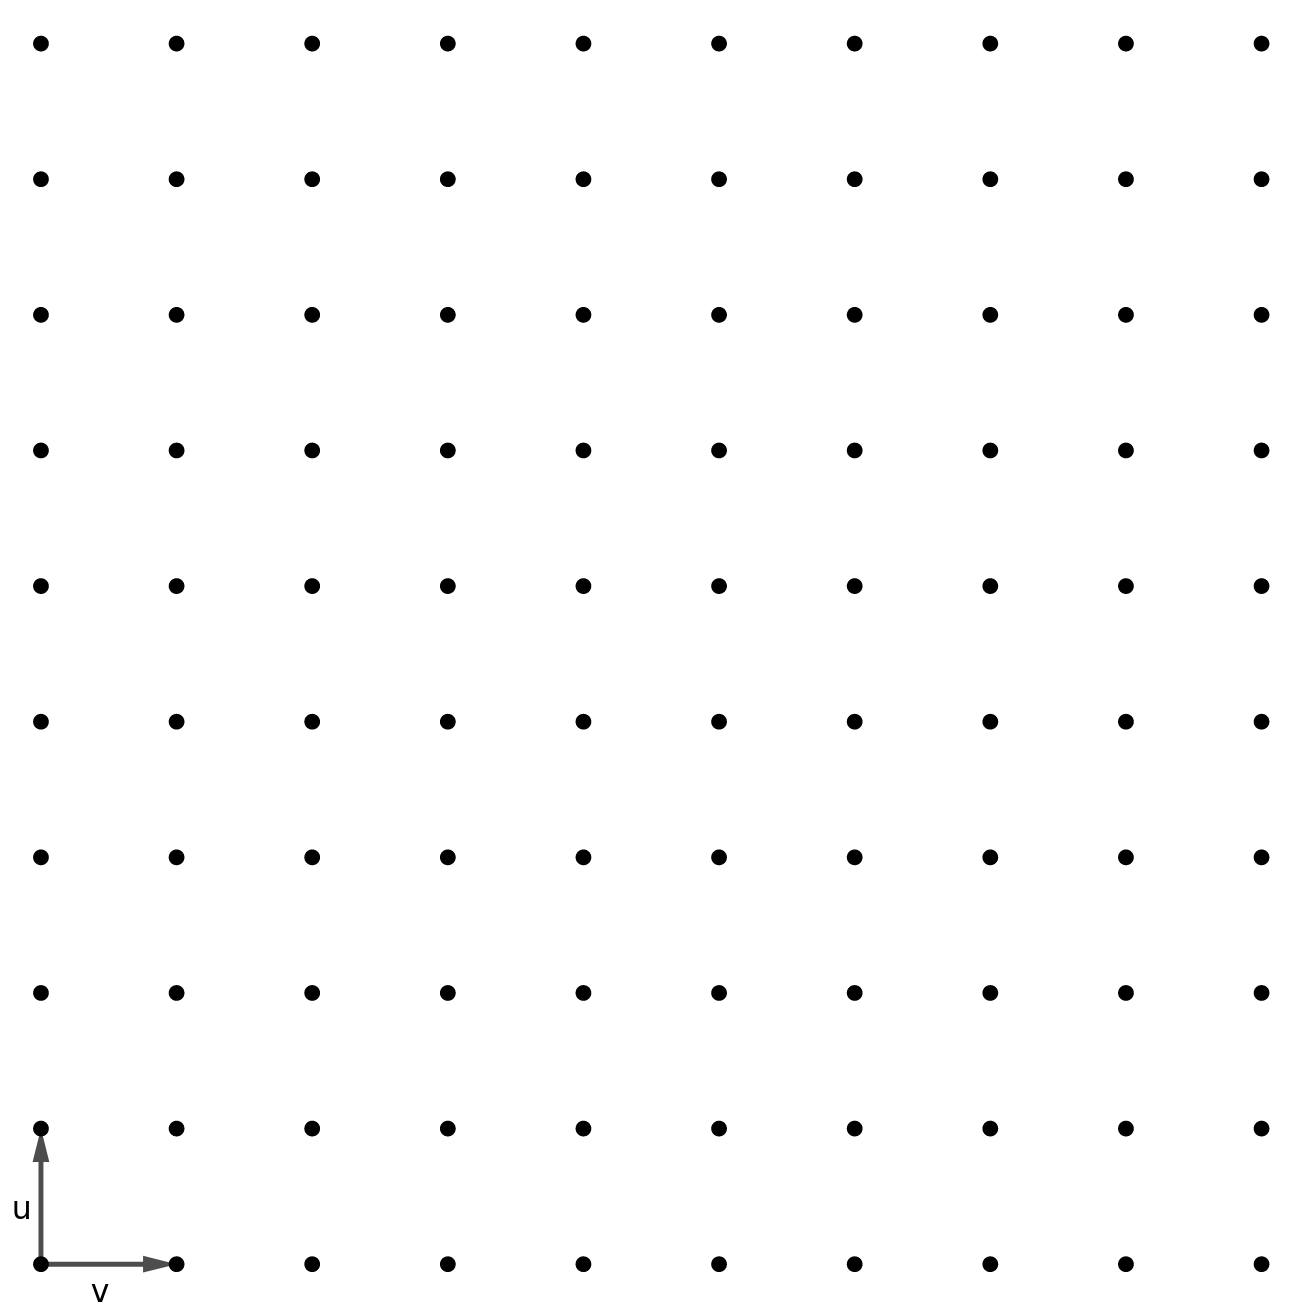
\includegraphics[width=0.75\textwidth]{Figuras/base_boa.png}\\
            \footnotesize{Fonte: O autor.}
            \label{fig:base_boa}
        \end{minipage}\hfill
        \begin{minipage}[c]{0.5\linewidth}
            \centering
            \caption{Exemplo de uma base ruim.}
            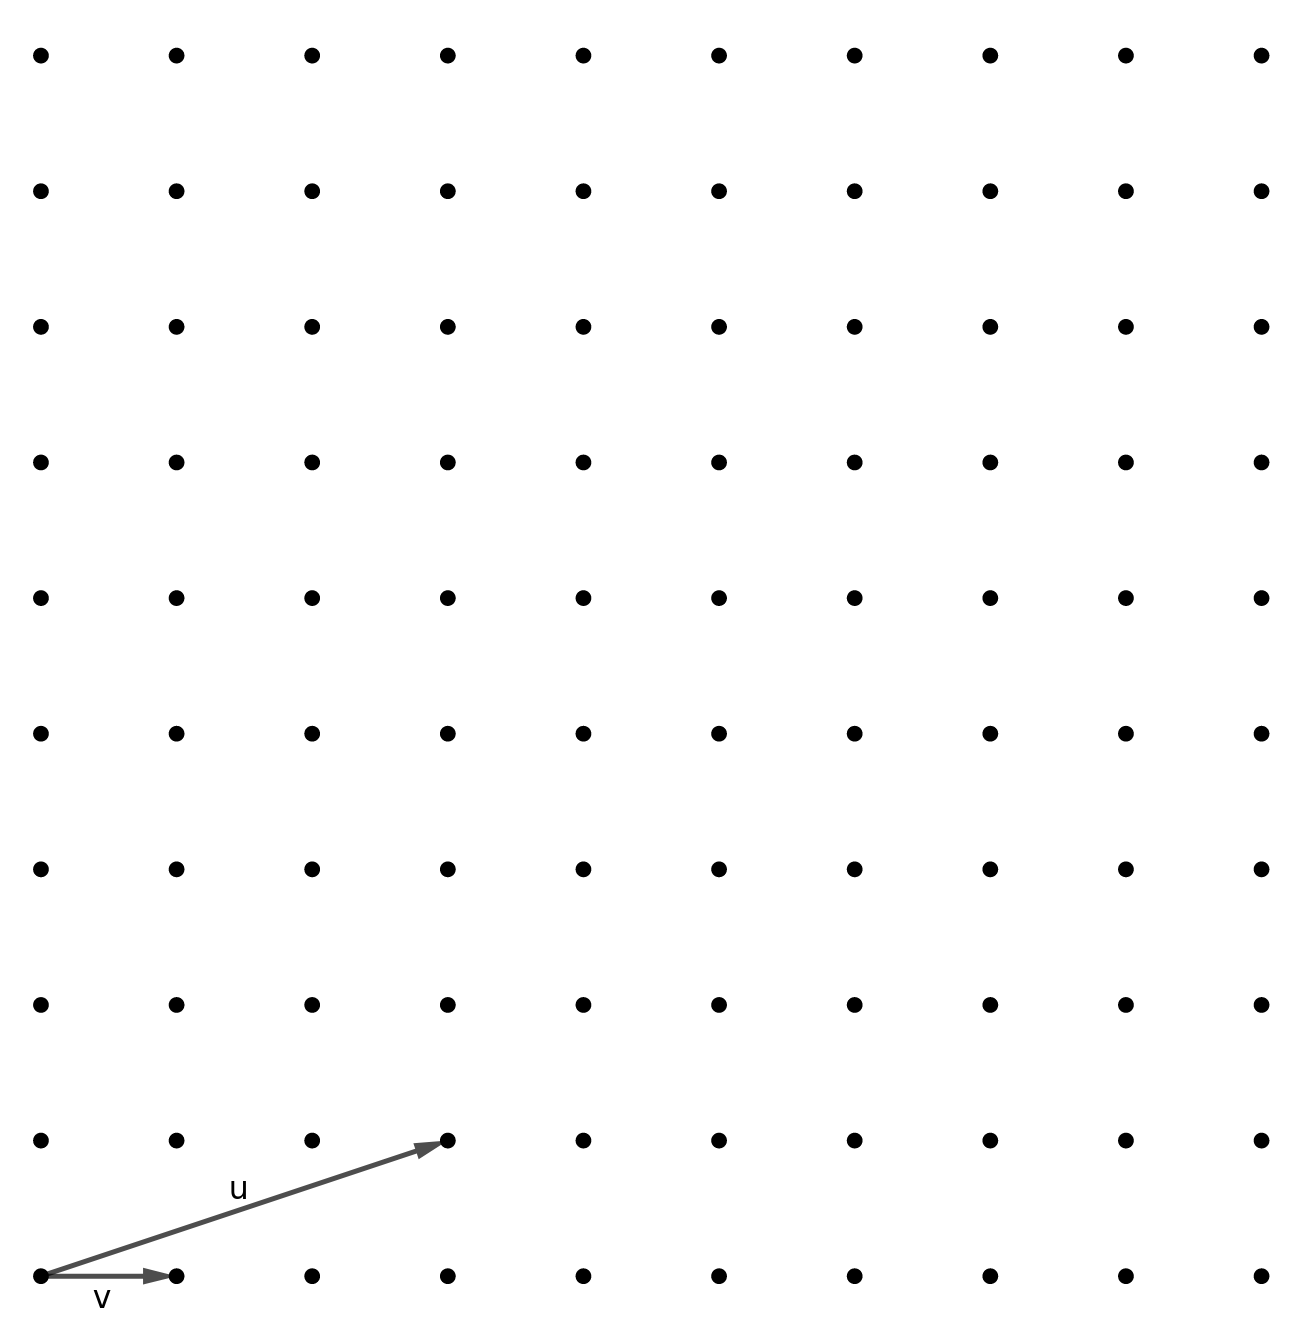
\includegraphics[width=0.75\textwidth]{Figuras/base_ruim.png}\\
            \footnotesize{Fonte: O autor.}
            \label{fig:base_ruim}
        \end{minipage}
    \end{figure}

    Os reticulados das Figuras \ref{fig:base_boa} e \ref{fig:base_ruim}, embora gerados por vetores completamente diferentes, são iguais tendo em vista que os vetores que geram o reticulado da Figura \ref{fig:base_ruim} podem ser expressos por uma combinação linear dos vetores que geram o reticulado da Figura \ref{fig:base_boa}. Entretanto, a base da Figura \ref{fig:base_boa}, gerada pelos vetores $\{(1,0),(0,1)\}$ é uma base boa, pois os vetores são ortogonais entre si e possuem sua norma pequena, a prova disso é o cálculo da \textit{Razão de Hadamard} da base, que é exatamente $1$. Já a base da Figura \ref{fig:base_ruim} é considerada ruim, visto que a \textit{Razão de Hadamard} é aproximadamente $0{,}56$. A base ser boa implica que conseguiremos boas aproximações pelos algoritmos de redução de base que serão abordados na seção \ref{algoritmos_reducao_base}.

    \subsection{Algoritmos de redução de base}
    \label{algoritmos_reducao_base}
        A razão pela qual deseja-se uma base reduzida, é para se obter uma boa aproximação para o problema \ac{CVP} através do algoritmo de Babai. O algoritmo de Babai \cite{babai} proposto em 1985 por László Babai, realiza uma aproximação da solução do problema CVP dada uma base boa, na qual este funciona da seguinte maneira:
        
        \begin{enumerate}
            \item Sendo $\vec{s} \notin \mathcal{L(\beta)}$, escreva $\vec{s}$ como uma combinação linear de $\beta$;
            \item Os coeficientes da combinação linear devem ser arredondados para um inteiro mais próximo;
            \item Os coeficientes arredondados combinados com a base devem gerar uma aproximação do vetor mais próximo de $\vec{s}$ que pertence à $\mathcal{L(\beta)}$.
        \end{enumerate}
        
        Esse algoritmo realiza uma boa aproximação do problema \ac{CVP} ao ter uma base bem ortogonal, do contrário, o resultado não é preciso. Tenha como exemplo um reticulado $\mathcal{L}(\beta)$ gerado pela base $\beta = \{ (5,1),(-2,8) \}$ e um vetor $\vec{s} = (27,8) \notin \mathcal{L}(\beta)$. A \textit{Razão de Hadamard} de $\beta$ é $\mathcal{H}(\beta) \thickapprox 0.999$, isso significa que devemos obter uma boa aproximação. Ao realizarmos os cálculos, obtém-se o vetor $\vec{c} = (30, 6)$, sendo relativamente próximo de $\vec{s}$. Agora, aplicando o algoritmo de Babai para outra base $\beta = \{(37,41),(103,113)\}$ menos ortogonal que gera o mesmo reticulado, em que  $\mathcal{H}(\beta) \thickapprox 0.07$, e que desejamos encontrar o vetor mais próximo de $\vec{s} = (27,8) \notin \mathcal{L}(\beta)$ obtém-se a seguinte aproximação $\vec{c} = -53(37,41) + 19(103,113) = (-4, -26)$. Perceba que a aproximação é pouco precisa com relação à anterior.
    
        Segundo \cite{barros} o algoritmo de Babai enxerga um vetor que não pertence a um reticulado dentro de um domínio fundamental, onde o resultado deste algoritmo estará no domínio fundamental deste vetor. Desta forma, quanto menos ortogonal for um domínio fundamental, mais distante do resultado ótimo este algoritmo pode retornar.

        Outro algoritmo importante é o de Gram-Schmidt, este algoritmo realiza sucessivas projeções entre pares de vetores da base com fim de retornar uma base com $\mathcal{H}(\beta) = 1$. Este algoritmo não retorna necessariamente uma base de vetores com coeficientes inteiros, visto que nem todo reticulado pode ser gerado por uma base totalmente ortogonal. Entretanto, este algoritmo é utilizado como subprocesso em outros algoritmos relacionados aos reticulados.

        \begin{algorithm}[!htbp]
            \SetAlgoLined
            \Entrada{$b_0,b_1,...,b_n \in \mathbb{R}^{m}$}
            \Saida{$b_0^{*},b_1^{*},...,b_n^{*} \in \mathbb{R}^{m}$}
            $b_0^{*} = \frac{b_0}{|b_0|}$\\
            \Para{$i \leftarrow 1$ até $n$}{
                \Para{$j \leftarrow 0$ até $i$}{
                    $b_i \leftarrow b_i - \langle b_i, b_j \rangle b_j$
                }
                $b_i^{*} \leftarrow \frac{b_i}{|b_i|}$
            }
            
            \Retorna{$b_0^{*},b_1^{*},...,b_n^{*}$}
        
            \caption{Algoritmo de Gram-Schmidt}
            \label{algo:gram_schmidt}
        \end{algorithm}
    
        O algoritmo \textit{Lenstra–Lenstra–Lovász} (LLL) \cite{lll} é um dos principais algoritmos de redução de base de reticulados. O Algoritmo LLL realiza uma aproximação da solução ótima dos problemas \ac{SVP} e \ac{CVP}. Para o problema \ac{SVP} o LLL realiza uma aproximação de $(2/\sqrt{3})^n \lambda_1$ em que $n$ é a dimensão do reticulado. Isto é, dada uma base, o algoritmo LLL irá encontrar um vetor que está a $(2/\sqrt{3})^n$ de distância máxima do vetor mais curto deste reticulado. E, para o \ac{CVP}, o LLL irá encontrar um vetor que está a uma distância de $2(2/\sqrt{3})^n$ do vetor alvo \cite{daniele-lattices}. O Algoritmo \ref{algo:lll} descreve o funcionamento do algoritmo LLL.\\    
        %Existem outros algoritmos de redução de base como...

        \begin{algorithm}[!htbp]
            \SetAlgoLined
            \Entrada{$ b_0,b_1,...,b_n \in \mathbb{Z}^{m}$, $\delta = \frac{3}{4}$}
            \Saida{$b_0,b_1,...,b_n \in \mathbb{Z}^{m}$}
            $\mu_{i,j} = \frac{b_i.b_{j}^{*}}{b_{j}^{*}.b_{j}^{*}}$\\
            \Inicio{
                
                $b_0^{*},b_1^{*},...,b_n^{*} \leftarrow$ Gram-Schmidt($b_0,b_1,...,b_n$)\\
                $k \leftarrow 1$\\
                \Enqto{$k \leq n$}{
                    \Para{$j \leftarrow k-1$ até $0$}{
                        \Se{$|\mu_{k,j}| > \frac{1}{2}$}{
                            $b_k \leftarrow b_k - \lfloor \mu_{k,j} \rceil b_j$\\
                            $b_0^{*},b_1^{*},...,b_n^{*} \leftarrow$ Gram-Schmidt($b_0,b_1,...,b_n$)\\
                        }
                    }
                    
                    \eSe{$\langle b_k^{*}, b_k^{*}\rangle > (\delta - \mu_{k,k-1}^{2})\langle b_{k-1}^{*}, b_{k-1}^{*}\rangle$}{
                        $k \leftarrow k + 1$\\
                    }{
                        Swap($b_k , b_k-1$)\\
                        $b_0^{*},b_1^{*},...,b_n^{*} \leftarrow$ Gram-Schmidt($b_0,b_1,...,b_n$)\\
                        $k \leftarrow Max(k-1, 1)$
                    }
                }
                
                \Retorna{$b_0,b_1,...,b_n$}
            }
            \caption{Algoritmo LLL}
            \label{algo:lll}
        \end{algorithm}

\section{Considerações finais do capítulo}
    Este capítulo apresenta a estrutura de reticulados e seus conceitos fundamentais, como também os principais problemas matemáticos envolvendo esta estrutura e as técnicas e algoritmos que resolvem estes problemas ou encontram uma solução aproximada do resultado ótimo. Estes conceitos, problemas e algoritmos estão relacionados com o algoritmo \ac{ML-KEM} apresentado no Capítulo \ref{cap:ml_kem}.